\documentclass[10pt,pdf,hyperref={unicode}, dvipsnames]{beamer}
%!TEX root = ../presentation.tex
\usepackage[english,russian]{babel}
% \usepackage[T2A,T1]{fontenc}
\usepackage[utf8]{inputenc}
% \usepackage{tikz}
\usepackage[unicode]{hyperref}
% \usepackage{pgfplots,standalone}
\usepackage{caption}
\usepackage[normalem]{ulem}
\usepackage
	{
		% Дополнения Американского математического общества (AMS)
		amssymb,
		amsfonts,
		amsmath,
		amsthm,
		physics
		}
% \usepackage{lmodern}
% \pgfplotsset{compat=newest} 
% \usetikzlibrary{%
%     decorations.pathreplacing,%
%     decorations.pathmorphing,%
%     patterns,%
%     angles,%
%     quotes,%
%     calc, %
%     3d, %
%     backgrounds, %
%     positioning%
% }


% Стиль презентации

 \usetheme{default}
 \usefonttheme{professionalfonts}
 \usecolortheme{}
 % \usecolortheme{whale}
% \let\oldframe\enumerate
% \renewcommand{\frame}{%
% \oldframe
% \let\olditemize\itemize
% \renewcommand\itemize{\olditemize\addtolength{\itemsep}{100pt}}%
% }
 

% \setbeamercolor{frametitle right}{fg=white,bg=Brown!85}
% \setbeamercolor{frametitle}{fg=white,bg=Brown!85}
%\setbeamercolor{frametitle right}{fg=white,bg=black!85} %
\setbeamercolor{frametitle}{fg=white,bg=black!85} % Цвет титульника
\setbeamercolor{item projected}{fg=white,bg=black!85} % Цвет титульника
\setbeamertemplate{blocks}[rounded][shadow=false] %стиль блоков
\setbeamertemplate{itemize item}{\color{black!85}$\bullet$}
\setbeamertemplate{headline}{}
\setbeamertemplate{footline}{} 
\setbeamertemplate{navigation symbols}{} % минус навигация
% \let\Tiny=\tiny % решает проблему со шрифтами в TexLive
%\setbeamertemplate
%	{footline}{
%		\color{black!40!white}
%		\quad\hfill
%		\insertframenumber/\inserttotalframenumber
%		\hfill\vspace{1cm}\quad
%	} 


\beamersetrightmargin{1cm} 
\beamersetleftmargin{1cm}

\setbeamertemplate{enumerate item}
{
	\usebeamercolor[bg]{item projected}
	\raisebox{1pt}{\colorbox{black!85}{\color{fg}\footnotesize\insertenumlabel}}%
}

% \setbeamertemplate{itemize item}{%
% 	\usebeamercolor[bg]{item projected}%
% 	\raisebox{3pt}{{\colorbox{black!85}\footnotesize$\bf$\bullet}}%
% }

\setbeamercolor{item projected}{bg=black,fg=white}
\setbeamercolor{title}{bg=black!85,fg=white}

\setbeamertemplate{frametitle}
{	
	\nointerlineskip
	\begin{beamercolorbox}[sep=15pt,ht=1.9em,wd=\paperwidth]{frametitle}
		% \vspace{}%
		\strut\insertframetitle\strut
		\vskip-1.8ex%	
	\end{beamercolorbox}
}


\usepackage{mathtools}
\mathtoolsset{showonlyrefs=true} 

\usepackage{import}
\usepackage{pdfpages}
\usepackage{transparent}
\usepackage{xcolor}
\usepackage{calc}

\newcommand{\executeiffilenewer}[3]{%
    \ifnum\pdfstrcmp{\pdffilemoddate{#1}}%
    {\pdffilemoddate{#2}}>0%
    {\immediate\write18{#3}}\fi%
}
\newcommand{\includesvg}[1]{%
    \executeiffilenewer{#1.svg}{#1.pdf}%
    {inkscape -z -D --file=#1.svg %
    --export-pdf=#1.pdf --export-latex}%
    \import{./fig/}{#1.pdf_tex}
}

\newcommand{\mean}[1]{\langle#1\rangle}
\usepackage{caption}
\usepackage{subcaption}
\renewcommand{\phi}{\varphi}
%\usepackage[e]{esvect}
%\usepackage{animate}
%\renewcommand{\vec}{\vv}
\newcommand{\tM}{\widetilde{M}}
\begin{document}
\title[Моделирование морской поверхности]{Численное моделирование морской поверхности}

\author{Понур К.А.}

\institute{Национальный исследовательский Нижегородский государственный университет имени Н. И. Лобачевского \\ Радиофизический факультет}

%!TEX root = ..\presentation.tex
\begin{frame}[plain]
	\begin{center}
		\small{\insertinstitute}
		\vspace{1cm}
	\end{center}
		\begin{beamercolorbox}[sep=8pt,center]{title}
			\usebeamerfont{title}\inserttitle
		\end{beamercolorbox}
		\vspace{0.1cm}
	\begin{flushright}
		\normalsize \textbf{Работу выполнил:}\\
		\large
		\insertauthor \\
		\vspace{0.5cm}
		\normalsize{\textbf{Научный руководитель:}\\}
		\large{Караев В.Ю.}
		\vfill
	\end{flushright}

	\centering{\small{\today }}
\end{frame}


% \section{Введение}
% \subsection{Цели работы}
\begin{frame}[t]
	\frametitle{Введение}
	\vfill
	\textbf{Цели: }\\
		% \vfill
		\begin{enumerate}
			% \item \sout{Получить зачёт по УНЭ.}
			\item Изучить принципы моделирования морской поверхности.

			\item Оптимизировать существующие алгоритмы.

            \item Предложить способы приближения моделируемой поверхности к
                реальной морской поверхности.
            \item Провести численный эксперимент на модельной поверхности с
                орбитальным радиовысотомером.
		\end{enumerate}
		\vfill
% \end{frame}
% \subsection{Актуальность работы}
% \begin{frame}[t]

	\textbf{Актуальность работы: }

	\begin{enumerate}
		% \item Проведение испытаний оборудования до его изготовления
		\item Тестирование и разработка алгоритмов восстановления океанографической информации
		\item Оценка возможностей новых радиолокаторов
		\item Постановка численных экспериментов, в частности накопление статистических данных
	\end{enumerate}
	\vfill
\end{frame}

% \begin{frame}[t]\frametitle{Основные понятия}

% Для статистически однородного и стационарного поля $\zeta$ высот морского волнения справедливо следующее выражение для его корреляционной функции:

% \begin{equation}
%  M(\rho) = \langle{\zeta(r)\zeta(r+\rho)}\rangle.
% \end{equation}

% Она связана с спектром высот $S(k)$ морской поверхности:
% \begin{equation}
%     	M(\rho)=\int\limits_0^{\infty} S(k)\cos(k \rho) \dd{k},
% \end{equation}    
% Спектр уклонов морской поверхности связан со спектром высот соотношением $S_{\theta}(k)=k^2 S(k)$.

% Корреляционная функция наклонов:
% \begin{equation}
% 	M_{\theta}(\rho)=\int\limits_0^{\infty} k^2 S(k)\cos(k \rho) \dd{k}
% \end{equation}
%     % Если поверхность представляем как $\zeta(r)= \sum\limits_{i=1}^N a_i\cos(k_i r+ \phi)$, то корреляционная функция модельного поля определяется выражением: 
%     % \begin{equation}
%     % 	\tM(\rho)=\sum\limits_0^{N} b_i \cos(k_i \rho), \quad b_i=\frac{a_i^2}{2},
%     % \end{equation}
%     % $k_i$ -- абсцисса спектральной компоненты
 
%     % $b_i$ -- ордината спектральной компоненты

% \end{frame}



\begin{frame}[t]

\frametitle{Двумерная модель поверхностного волнения}


\begin{equation}
    \label{eq:surface2d}
    z(\vec r,t) = \sum\limits_{n=1}^{N} \sum\limits_{m=1}^{M}
    A_n(\kappa_n) \cdot
    F_{nm}(\kappa_n,\phi_m) \cos \qty(\omega_n t + \vec \kappa_n \vec r + \psi_{nm}),
\end{equation}
\footnotesize
где $\psi_{nm}$ -- случайная фаза, равномерно распределенная в интервале от
$-\pi$
до $ \pi$, 

$F_m(\kappa_n, \phi_m)$ -- азимутальное
распределение для гармоники с волновым числом  $\kappa_n$,  

$\vec \kappa_n =
(\kappa_{nx}, \kappa_{ny})$ -- 
волновой вектор. 

\begin{columns}[t]
    \begin{column}{0.49\linewidth}
    \footnotesize
    \begin{equation}
        \label{eq:Amplitude}
        A_n(\kappa_n) = \frac{1}{2 \pi} \sqrt{\int\limits_{\Delta \kappa_n} 2
            S(\kappa)
        \dd \kappa},
    \end{equation}
     где  $S(\kappa)$  - спектральная плотность
    мощности,

    \begin{equation}
        F_{nm}(\kappa_n,\phi_m) = \sqrt{\int\limits_{\Delta \phi_m}
        \Phi_{\xi}(\kappa_n,\phi) \dd \phi},
        \end{equation}
     где  $\Phi(\kappa_n, \phi)$   -- { азимутальная плотность
        мощности}
    \end{column}
    \begin{column}[T]{0.49\linewidth}
        \footnotesize
        Теоретическая корреляционная функция
        \begin{equation}
            K(\rho) = \int\limits_{-\infty}^{\infty} S(\kappa) e^{i \kappa
            \rho}\dd  \kappa
        \end{equation}
        Корреляционная функция модельной поверхности
        \begin{equation}
            \tilde K(\rho) = \sum\limits_{n=1}^{N} \frac{A_n^2}{2} \cos(\kappa \rho)
        \end{equation}
        Критерий качества моделирования
        \begin{equation}
            \tilde K(\rho) \longrightarrow K(\rho)
        \end{equation}
    \end{column}
\end{columns}
\end{frame}
\begin{frame}[t]{}
    Определение высот, определение наклонов, определение наклонов по x,
    определение уклонами по y,
    \begin{equation}
        z(\vec r,t) = \sum\limits_{n=1}^{N} \sum\limits_{m=1}^{M}
        A_n(\kappa_n) \cdot
        F_{nm}(\kappa_n,\phi_m) \cos \qty(\omega_n t + \vec \kappa_n \vec r + \psi_{nm}),
    \end{equation}
    Определение уклонов в проекции на оси
    \begin{equation}
        \pdv{z(\vec r,t)}{x} = \zeta_x = \sum\limits_{n=1}^{N} \sum\limits_{m=1}^{M}
        A_n(\kappa_n) \cdot \kappa_{nx} \cdot
        F_{nm}(\kappa_n,\phi_m) \cos \qty(\omega_n t + \vec \kappa_n \vec r + \psi_{nm}),
    \end{equation}
    \begin{equation}
        \pdv{z(\vec r,t)}{y} = \zeta_y = \sum\limits_{n=1}^{N} \sum\limits_{m=1}^{M}
        A_n(\kappa_n) \cdot \kappa_{ny} \cdot
        F_{nm}(\kappa_n,\phi_m) \cos \qty(\omega_n t + \vec \kappa_n \vec r + \psi_{nm}),
    \end{equation}

    Определение полных уклонов
    \begin{equation}
        \zeta = \sqrt{\zeta_x^2 + \zeta_y^2}
    \end{equation}

    Определение орбитальной скорости
    \begin{equation}
         \pdv{z(\vec r,t)}{t} = v(\vec r, t) = \sum\limits_{n=1}^{N} \sum\limits_{m=1}^{M}
        A_n(\kappa_n) \cdot \omega_{n} \cdot
        F_{nm}(\kappa_n,\phi_m) \cos \qty(\omega_n t + \vec \kappa_n \vec r + \psi_{nm})
    \end{equation}
    
\end{frame}

\begin{frame}[t]{Метод <<отбеливания>> спектра}
    \begin{figure}[h!]
        \centering
        \begin{subfigure}{0.49\linewidth}
            \centering
            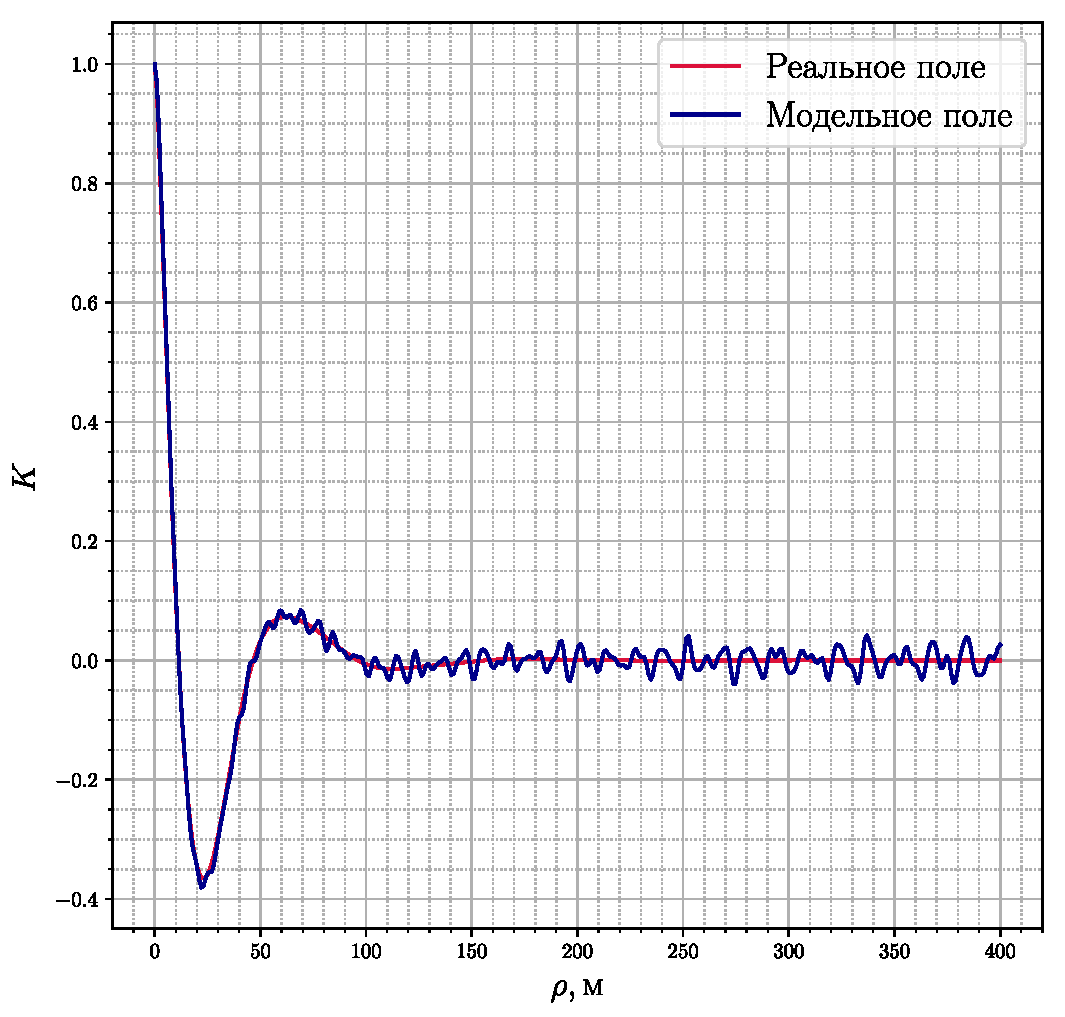
\includegraphics[width=\linewidth]{fig/correlation_height_height2.pdf}
        \end{subfigure}
        \begin{subfigure}{0.49\linewidth}
            \centering
            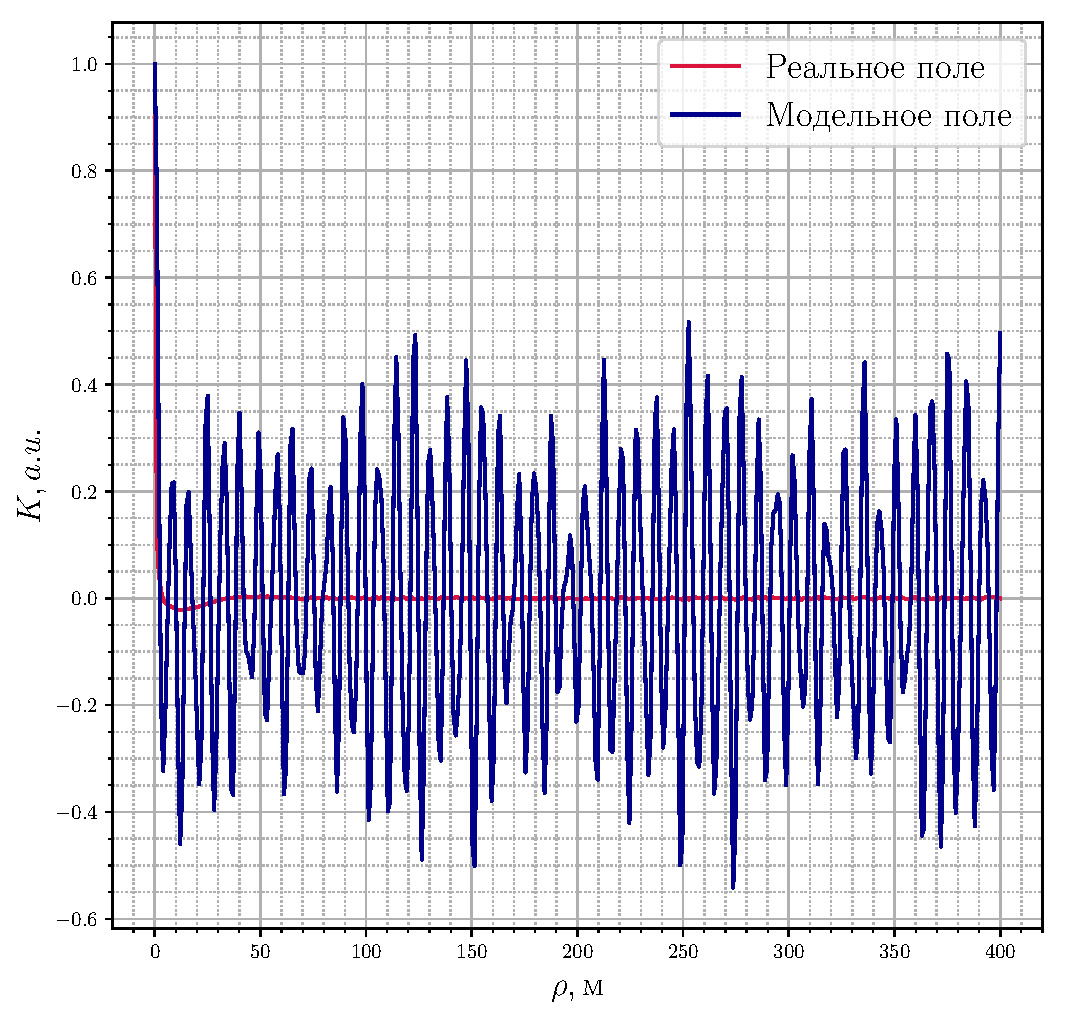
\includegraphics[width=\linewidth]{fig/correlation_angles_height2.pdf}
        \end{subfigure}
        \label{fig:ki}
    \end{figure}
\end{frame}

\begin{frame}[t]{Метод <<отбеливания>> спектра}
\begin{minipage}{0.49\linewidth}
    \centering
    Для высот:
\begin{equation}
    \footnotesize
    \kappa_i = \sqrt{\frac{N}{\int\limits_{-\infty}^{\infty} S(\kappa)
    \dd \kappa}} \cdot \int\limits_{\Delta k_i} \kappa^2
        S(\kappa) \dd \kappa, 
\end{equation}

\end{minipage}
\hfill
\begin{minipage}{0.45\linewidth}
    \centering
    Для уклонов: 
\begin{equation}
    \footnotesize
    \kappa_i = \sqrt{\frac{N}{\int\limits_{-\infty}^{\infty} \kappa^2 S(\kappa)
    \dd \kappa}} \cdot \int\limits_{\Delta k_i} \kappa^4
        S(\kappa) \dd \kappa. 
\end{equation}
\end{minipage}
\begin{figure}[h!]
    \begin{subfigure}{0.45\linewidth}
        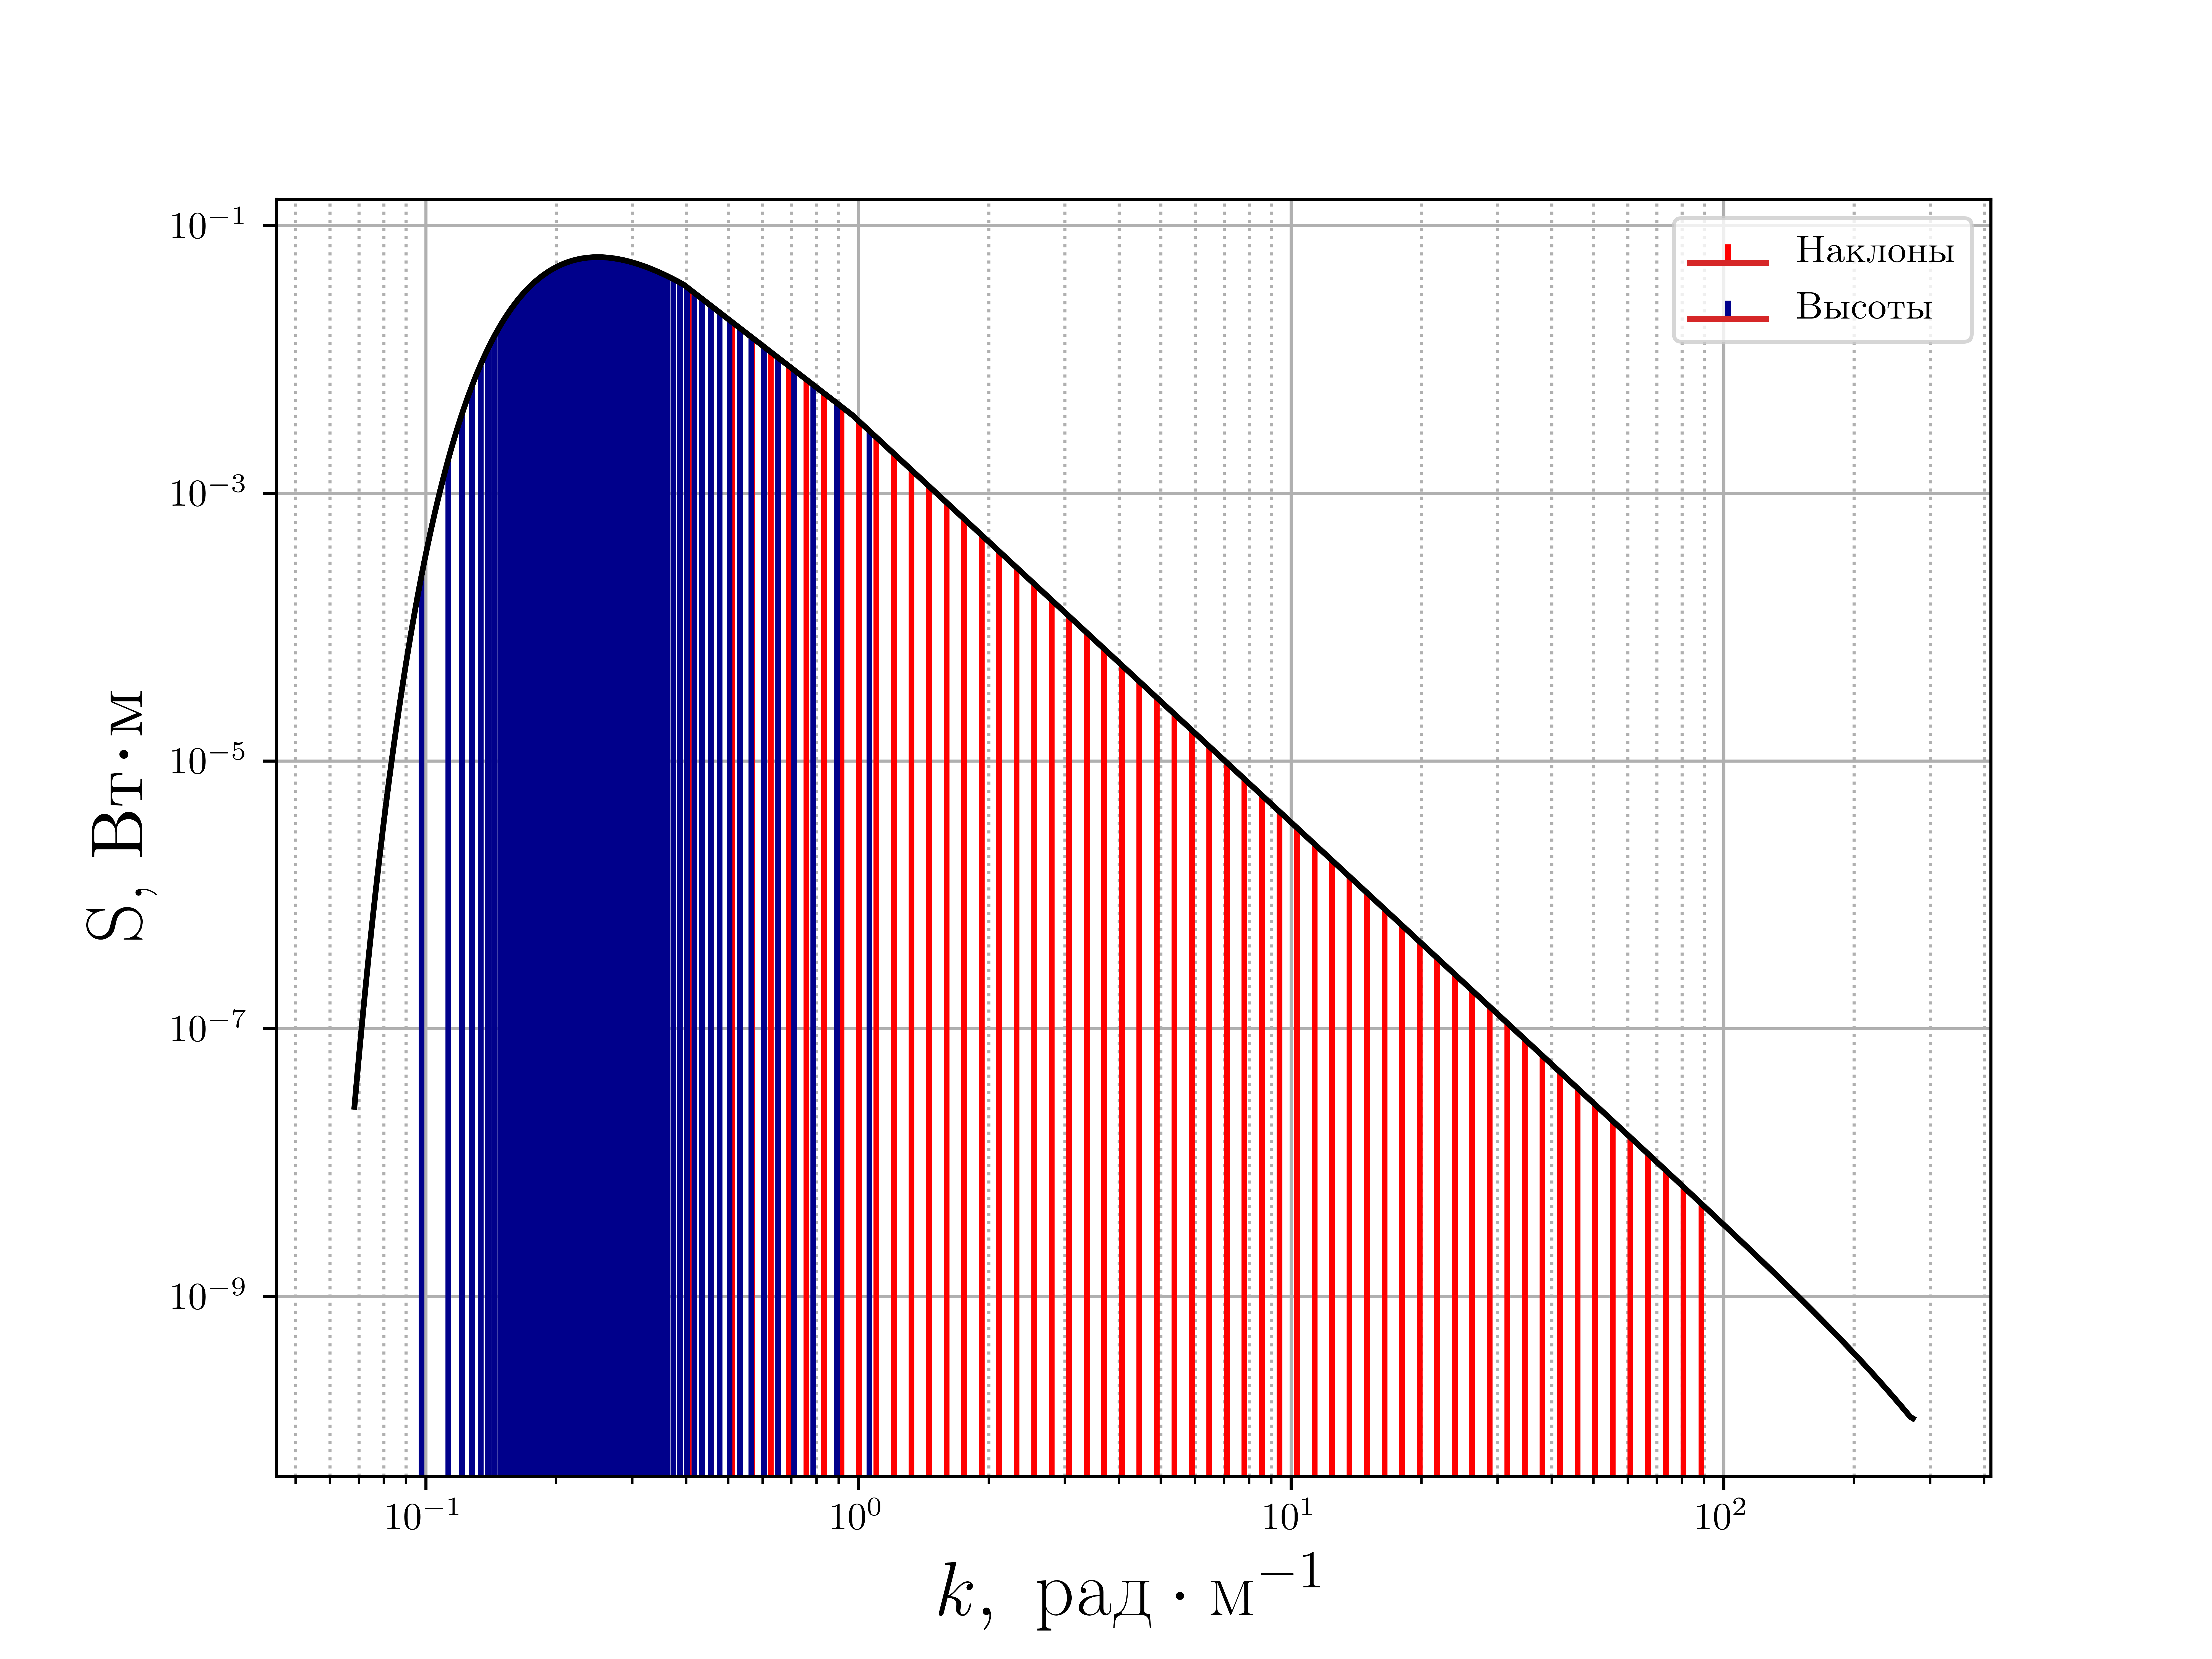
\includegraphics[width=\linewidth]{fig/fig3}
        \caption*{\footnotesize Расположение гармоник в области пространственных частот по
        методу отбеливания спектра, синим цветом обозначены гармоники,
    обеспечивающие минимум шума для корреляционной функции высот, красным --
для уклонов}
    \end{subfigure}
    \hfill
    \begin{subfigure}{0.49\linewidth}
        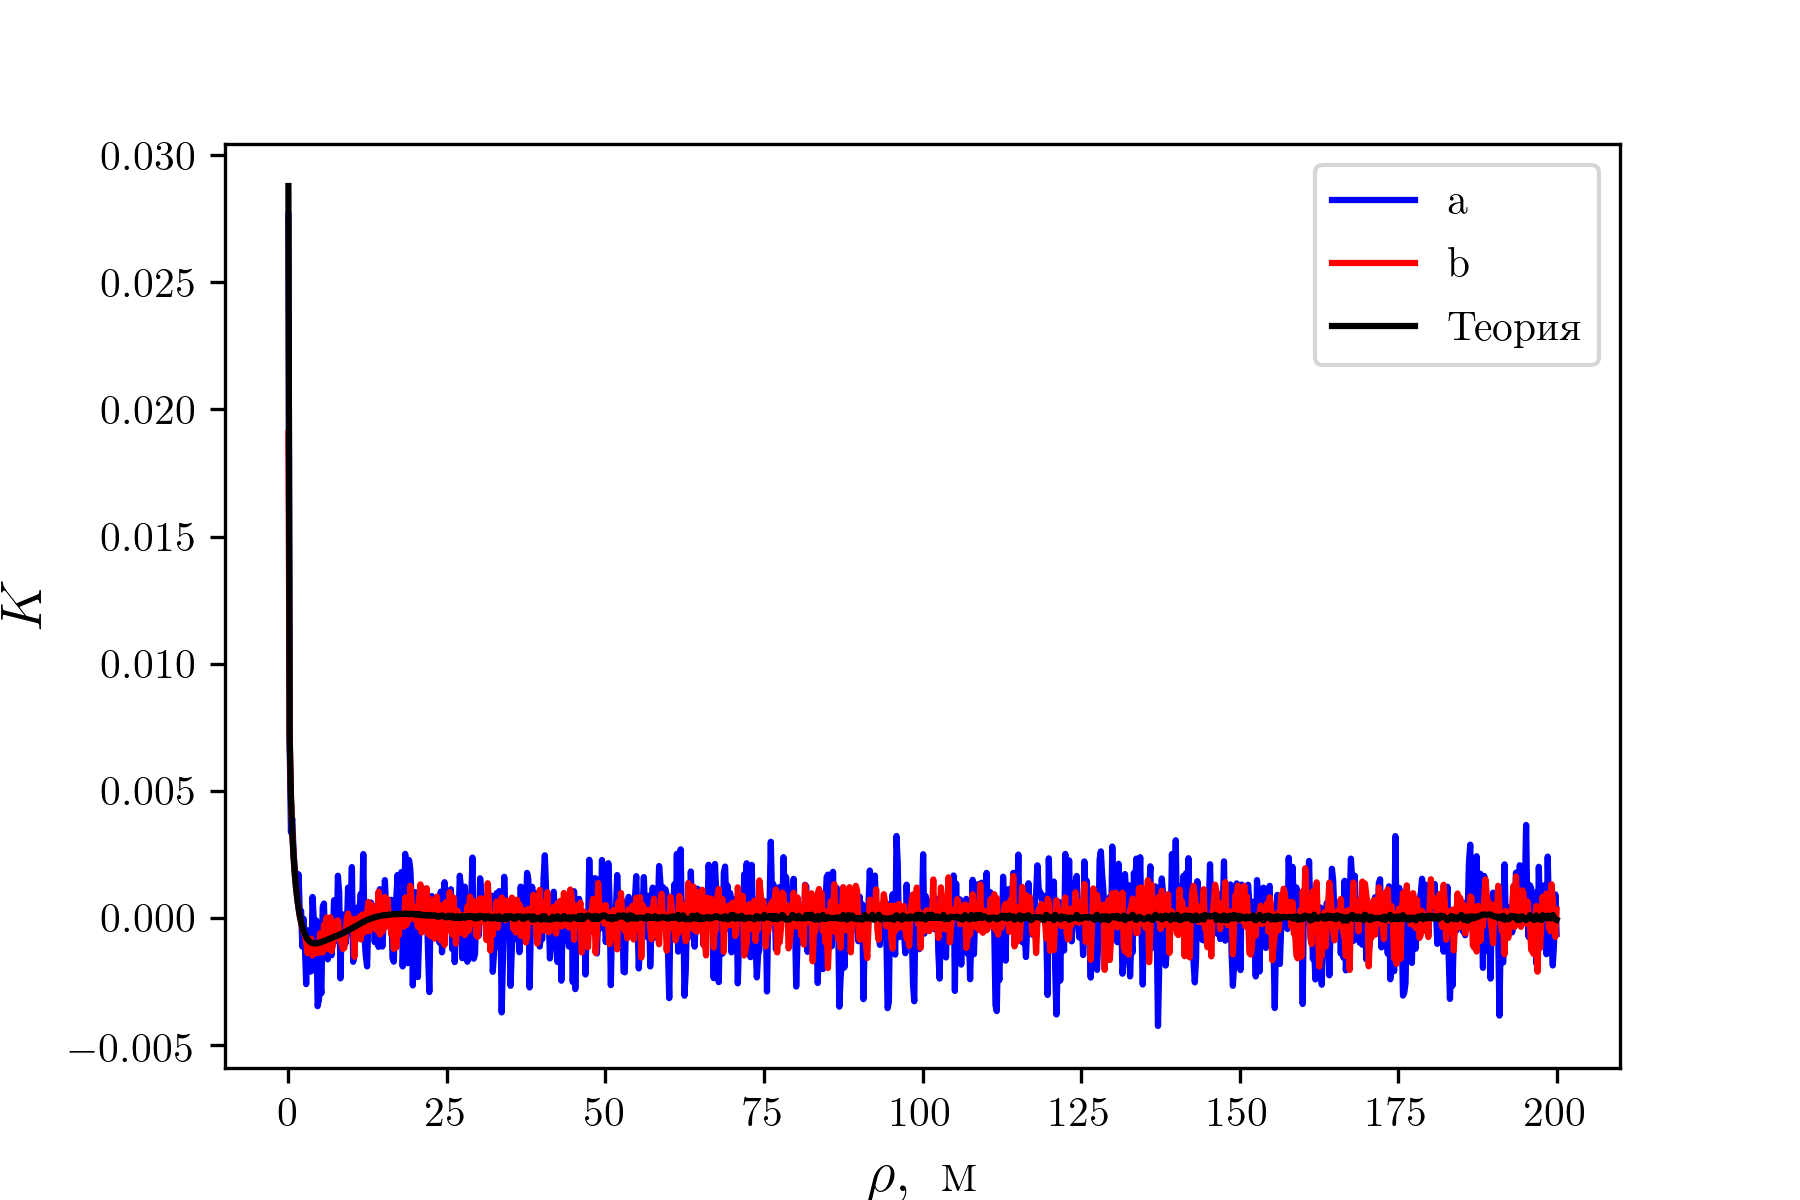
\includegraphics[width=\linewidth]{fig/water/whitening}
        \caption*{\footnotesize Корреляционная функция наклонов для различного расположения
        гармоник в частотной области: (a) логарифмическое распределение, (b)
    метод <<отбеливания>> спектра}
    \end{subfigure}
\end{figure}
\end{frame}

\begin{frame}[t]{Изображение поверхностей}
    \begin{figure}[h]
        \begin{subfigure}{0.49\linewidth}
            \centering
            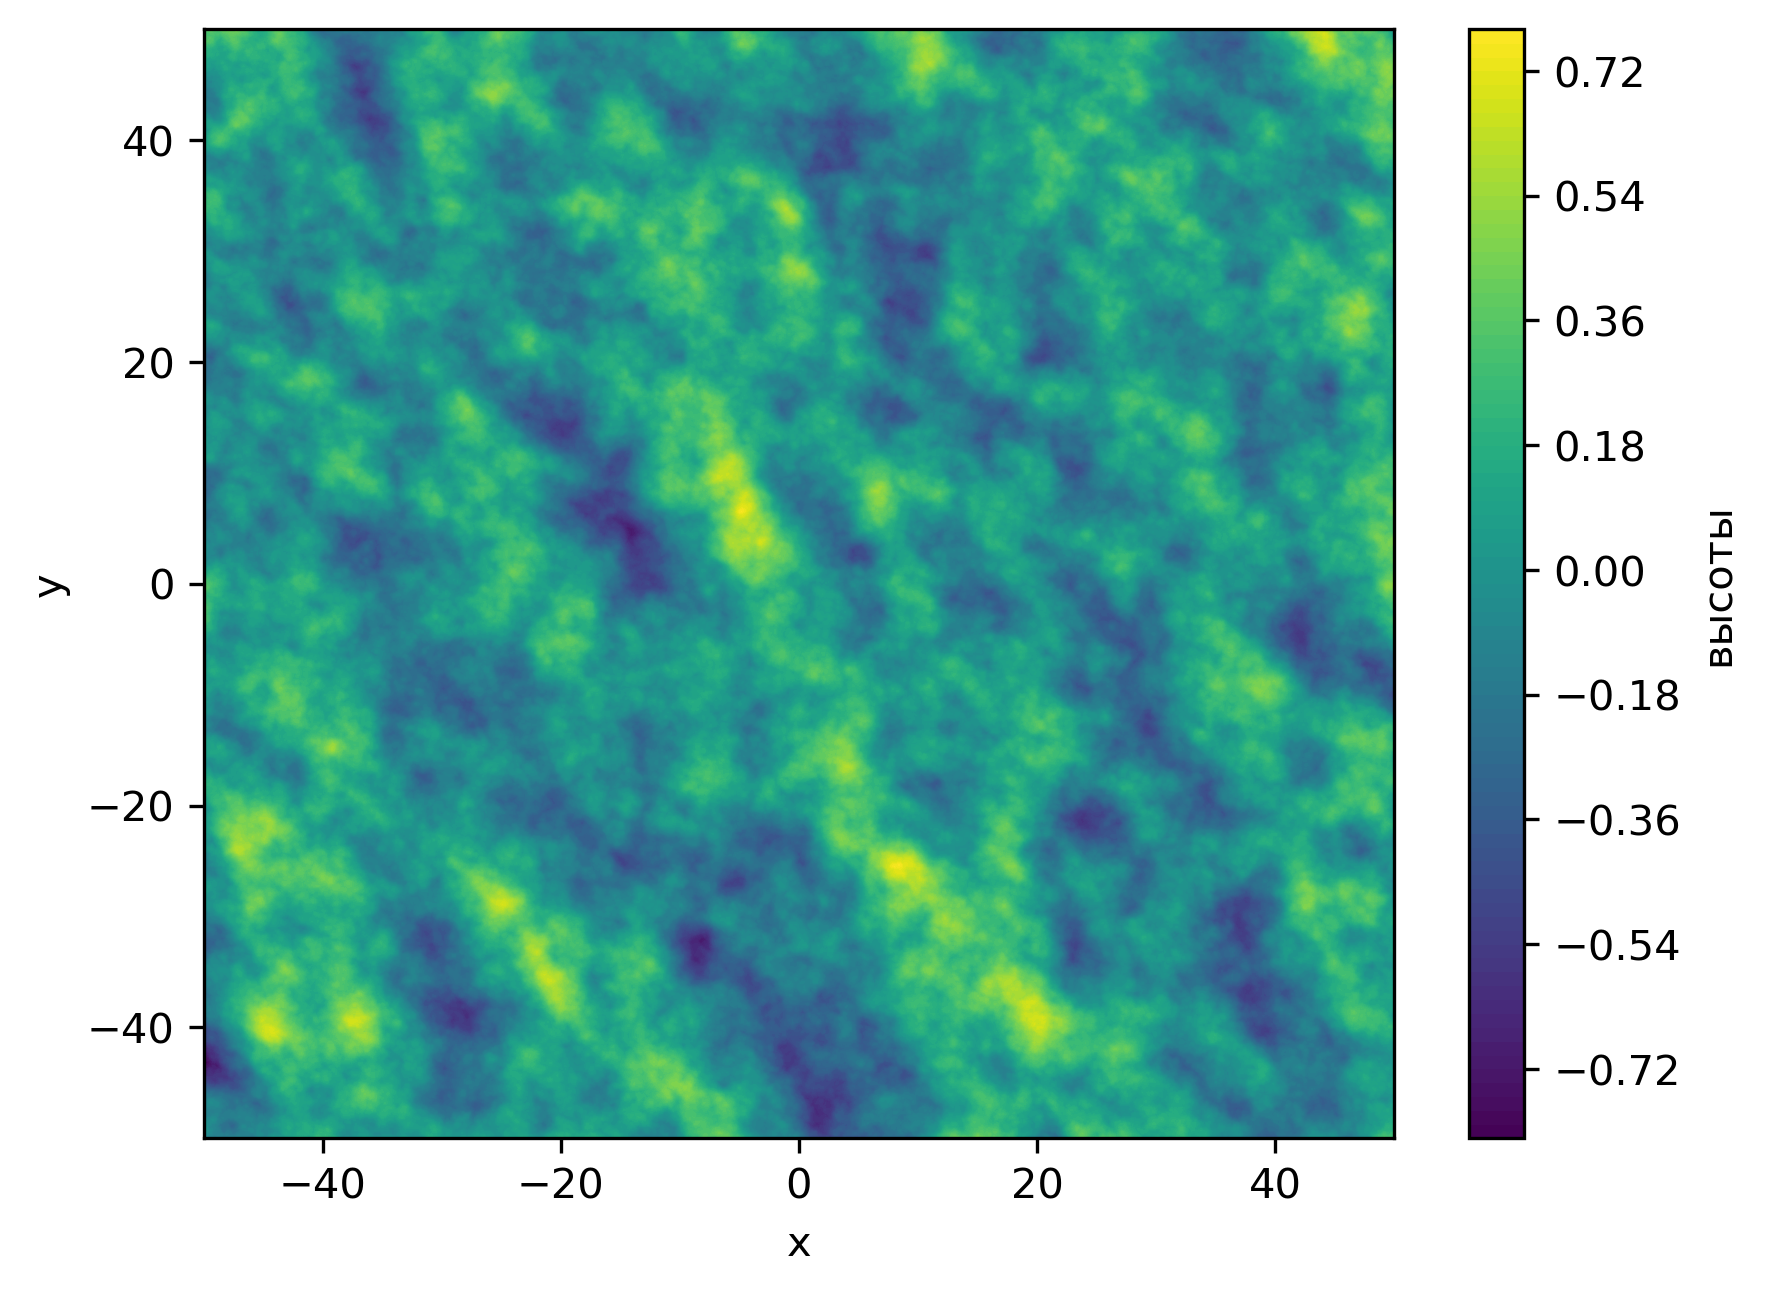
\includegraphics[width=1\linewidth]{img/heights}
        \end{subfigure}
        \begin{subfigure}{0.49\linewidth}
            \centering
            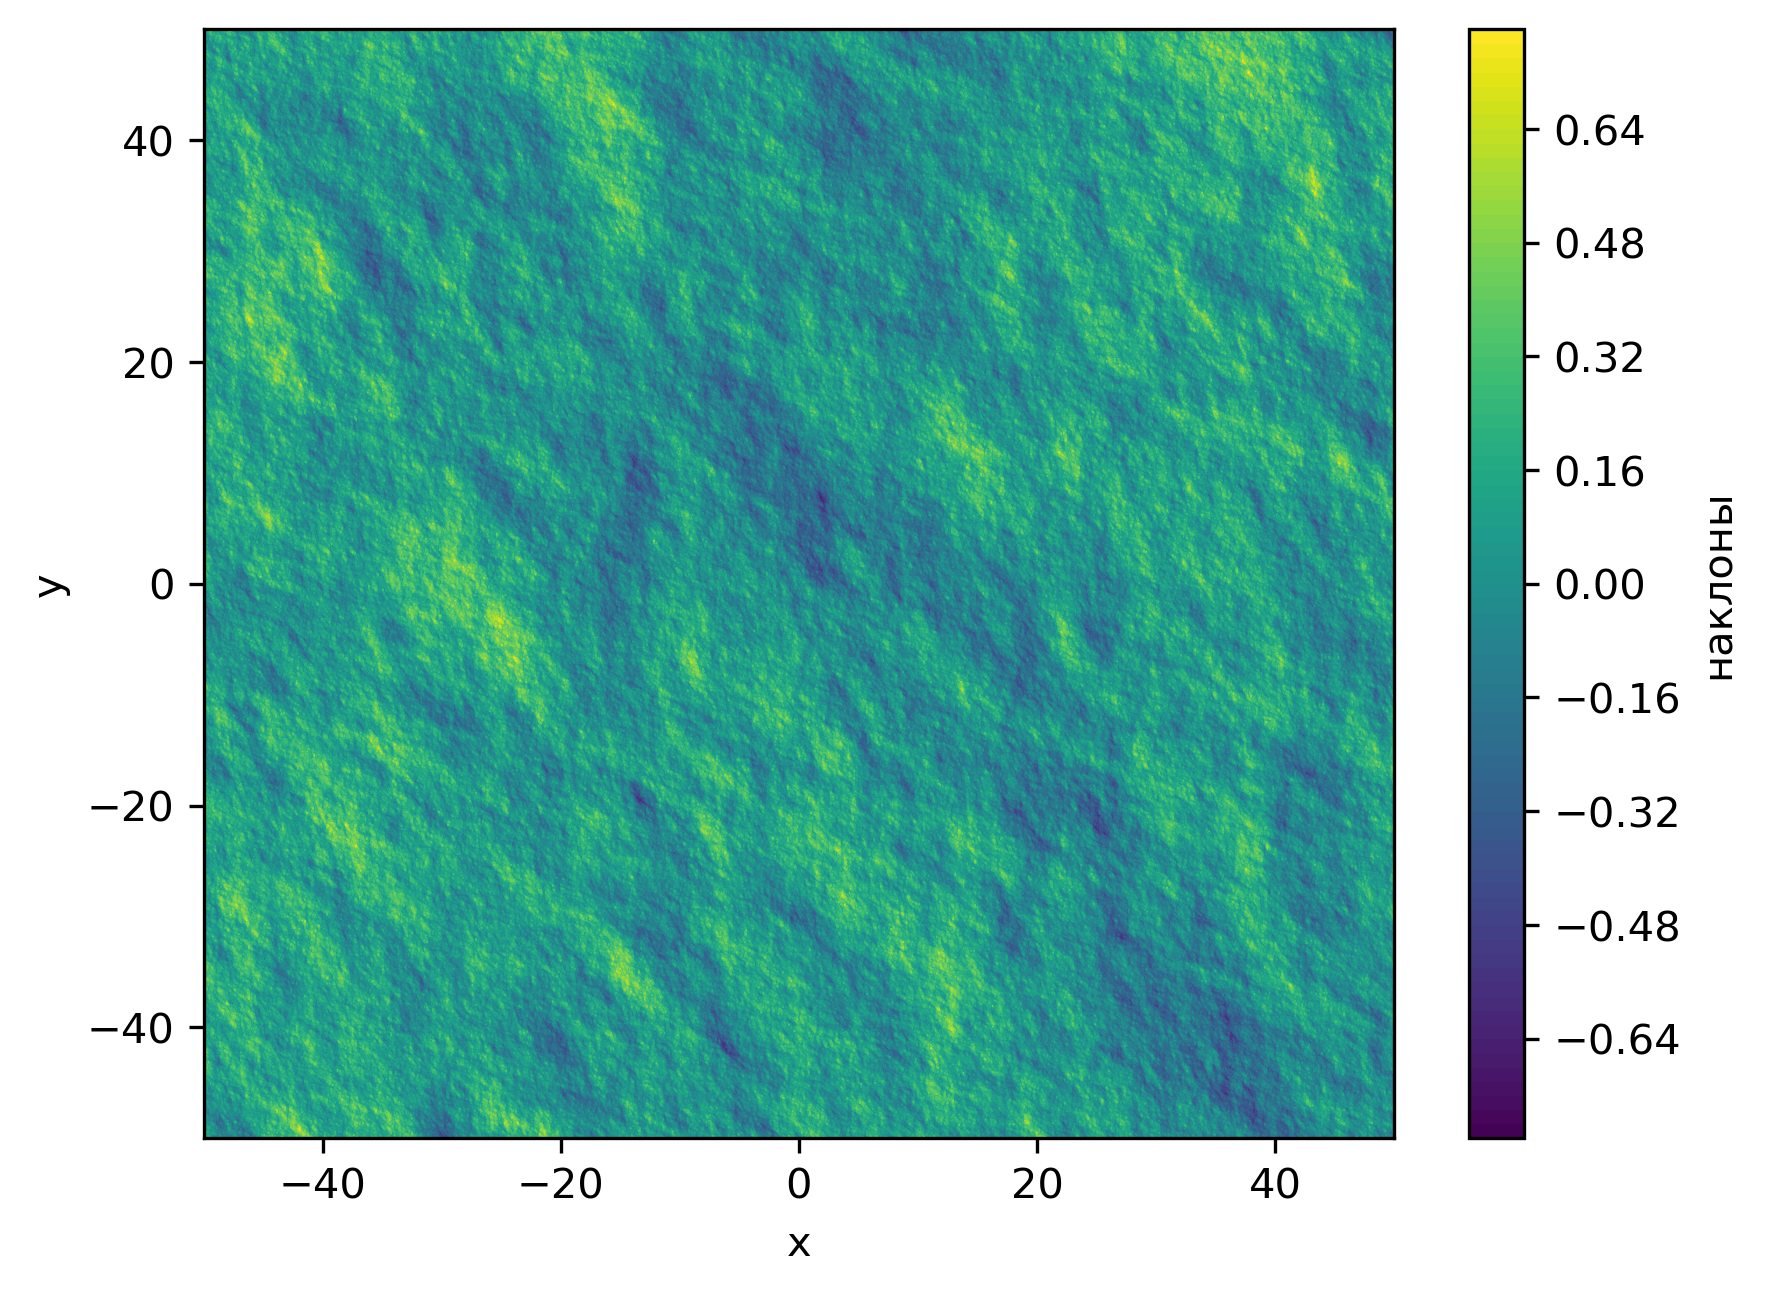
\includegraphics[width=1\linewidth]{img/slopes}
        \end{subfigure}
        \begin{subfigure}{0.49\linewidth}
            \centering
            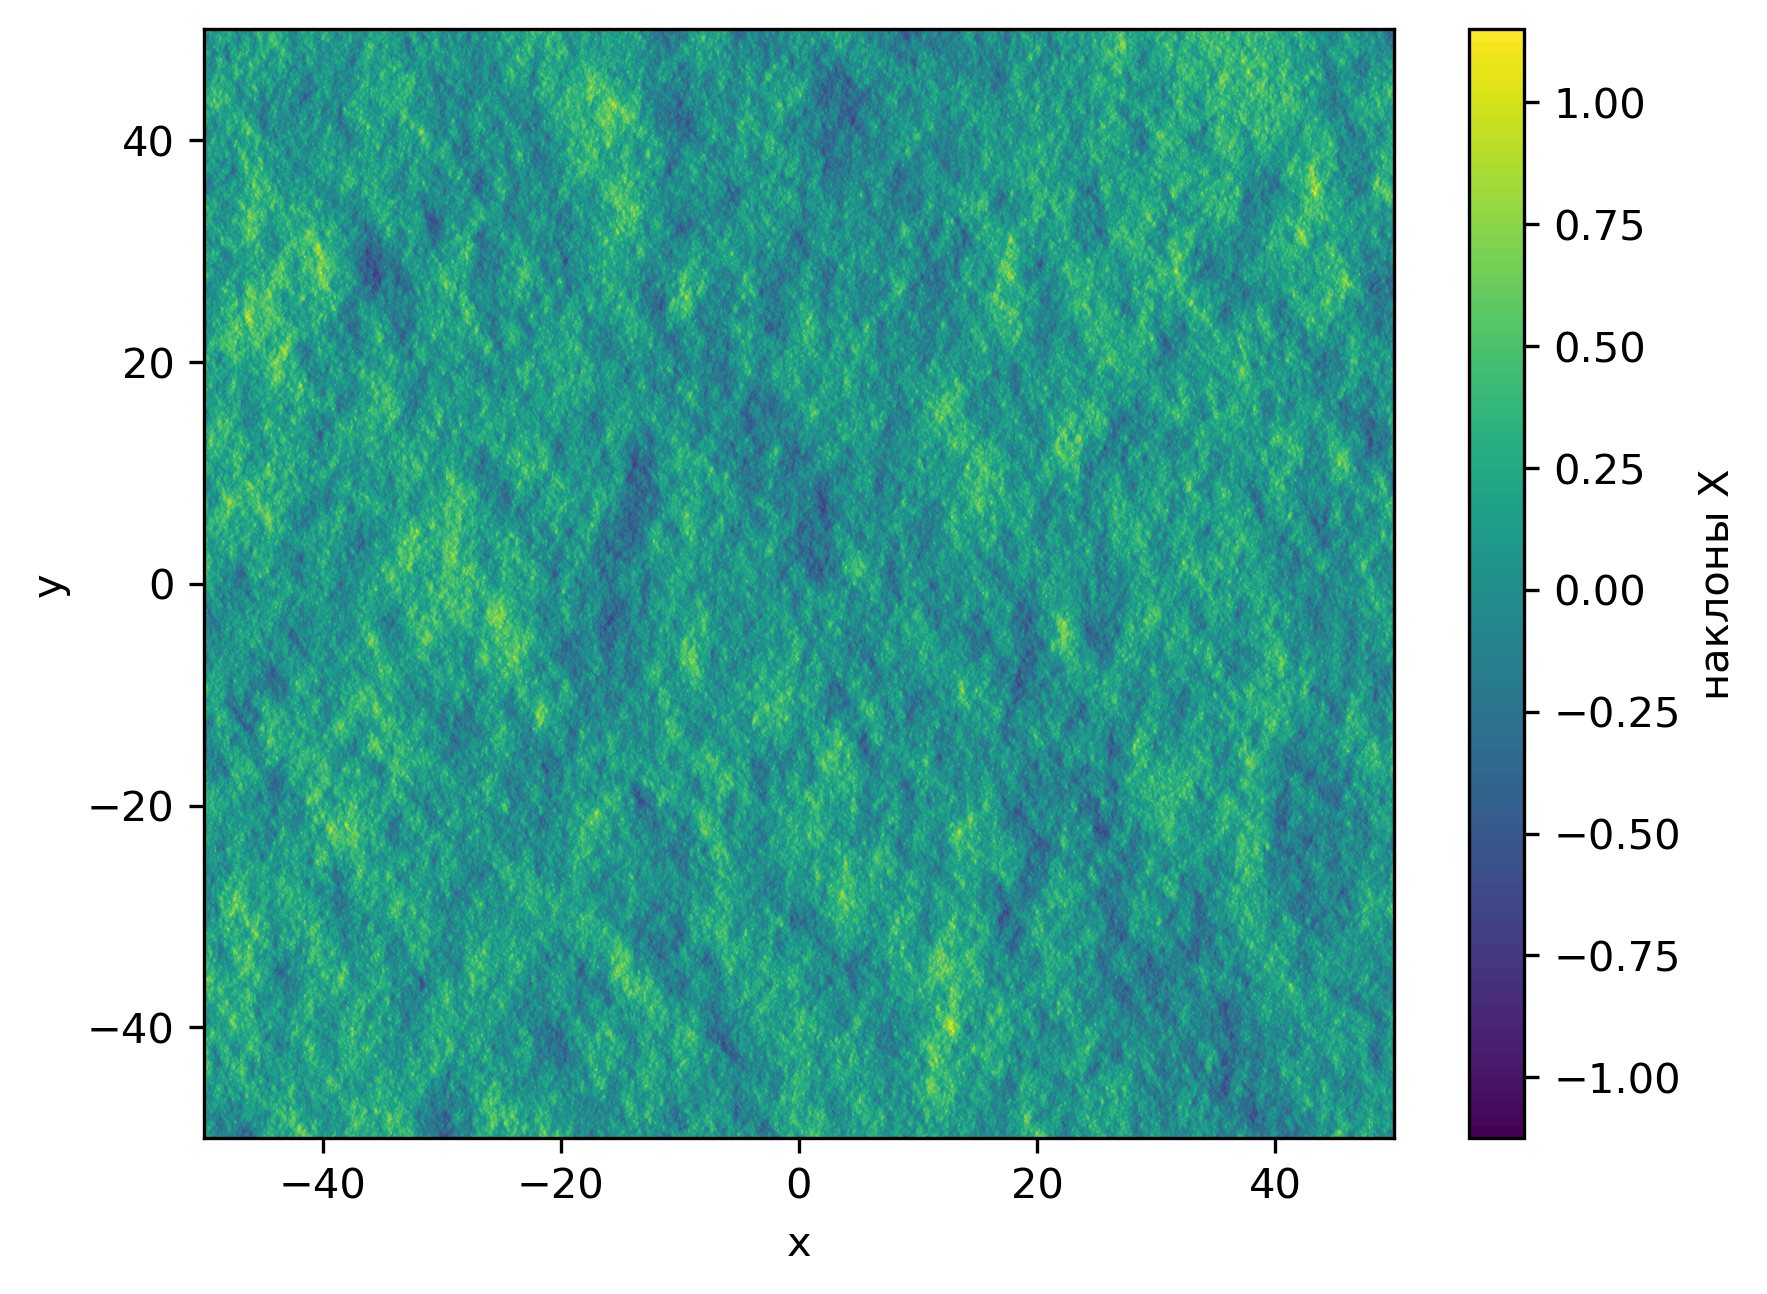
\includegraphics[width=1\linewidth]{img/slopesxx.png}
        \end{subfigure}
        \begin{subfigure}{0.49\linewidth}
            \centering
            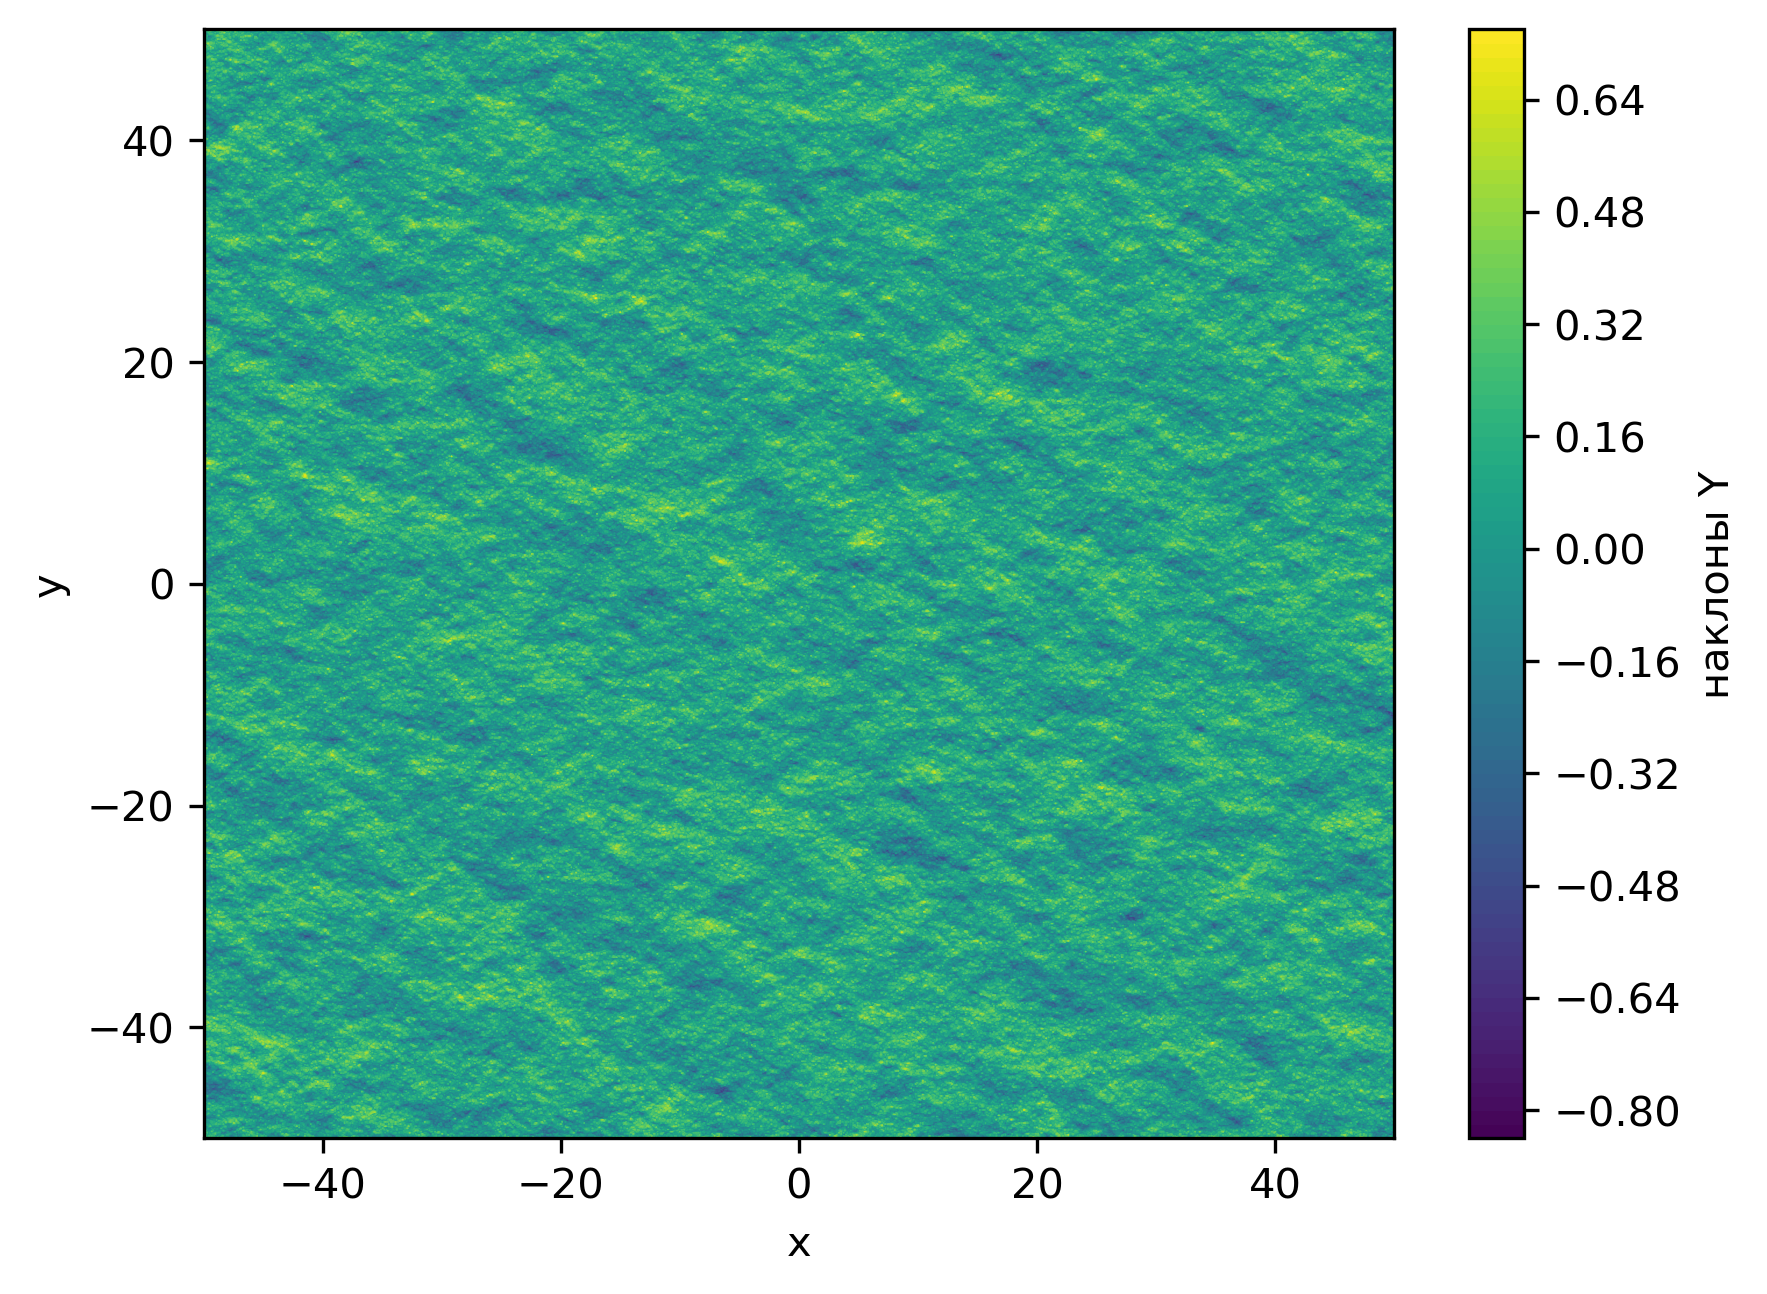
\includegraphics[width=1\linewidth]{img/slopesyy}
        \end{subfigure}
    \end{figure}    
\end{frame}

\begin{frame}[t]
	\frametitle{Увеличение производительности}
    Увеличение производительности достигается за счет библиотеки Numba, в
    которую входит JIT-компилятор с открытым исходным кодом,
    переводящий подмножество Python и NumPy в быстрый машинный код
    \begin{figure}[h]
        \begin{subfigure}{0.49\linewidth}
            \centering
            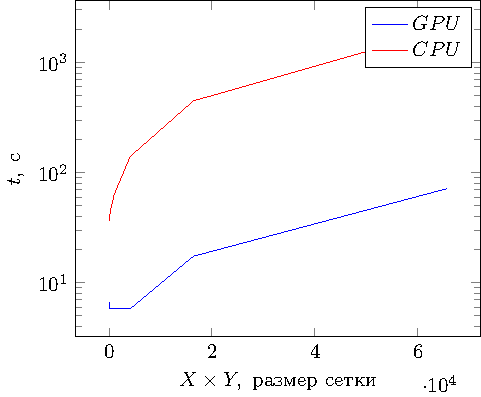
\includegraphics[width=\linewidth]{fig/water/gpucpu.pdf}
        \end{subfigure}
        \begin{subfigure}{0.49\linewidth}
            \centering
            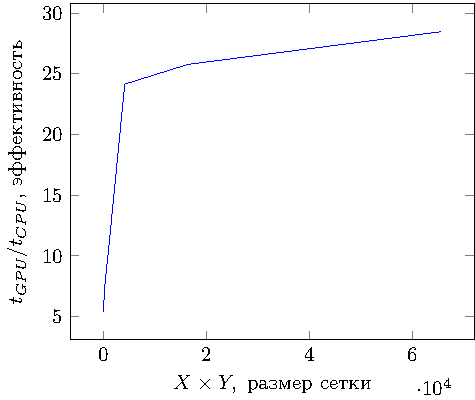
\includegraphics[width=\linewidth]{fig/water/gpucpu1.pdf}
        \end{subfigure}
    \end{figure}
    Используемое оборудование: 

    NVIDIA GeForce GTX 1660 (GPU),
    Intel Core i5-2400 (CPU)
\end{frame}
\begin{frame}[t]
    \frametitle{Модель заостренной поверхности}
    \begin{equation}
        \footnotesize
        \begin{cases}
            \label{eq:surface2dcwm}
            z(\vec r,t) = \sum\limits_{n=1}^{N} \sum\limits_{m=1}^{M}
            A_n(\kappa_n) \cdot
            F_m(\kappa_n,\phi_m) \cos \qty(\omega_n t + \vec \kappa_n \vec r_0 +
            \psi_{nm}),    \\
            x = x_0 - \sum\limits_{n=1}^{N} \sum\limits_{m=1}^{M}
            A_n(\kappa_n) \cdot
            F_m(\kappa_n,\phi_m) \cos\phi_m \sin\qty(\omega_n t + \vec \kappa_n \vec r_0 +
            \psi_{nm}),\\
            y = y_{0} - \sum\limits_{n=1}^{N} \sum\limits_{m=1}^{M}
            A_n(\kappa_n) \cdot
            F_m(\kappa_n,\phi_m) \sin \phi_m \sin \qty(\omega_n t + \vec \kappa_n \vec
            r_0 + \psi_{nm}),
        \end{cases}
    \end{equation}
    где $\vec \kappa$ -- двумерный волновой вектор,  
    $\vec r_0 = (x_0, y_0)$, $\vec r = (x, y)$

    \begin{figure}
        \centering
        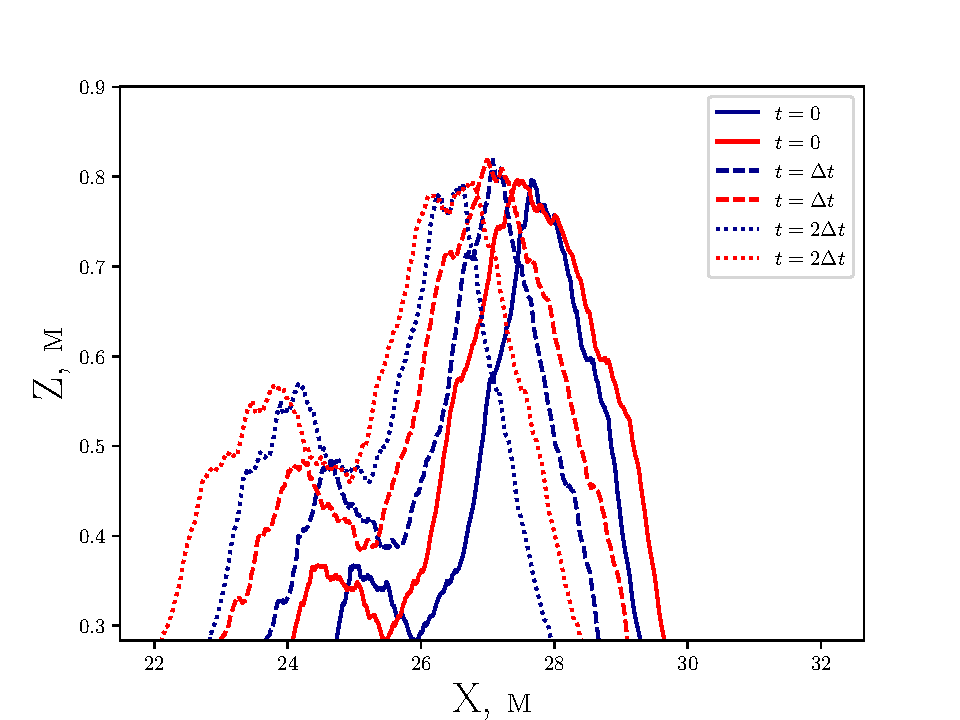
\includegraphics[height=0.5\textheight]{fig/evolution}
    \end{figure}
\end{frame}
\begin{frame}[t]
	\frametitle{Модель заостренной поверхности}
    \begin{figure}[h]
        \begin{subfigure}{0.49\linewidth}
            \centering
            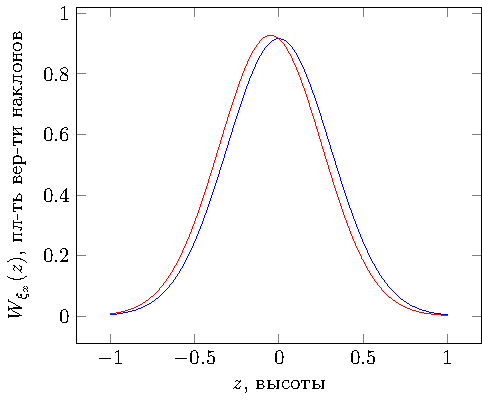
\includegraphics[width=\linewidth]{fig/water/pdf_cwm}
        \end{subfigure}
        \begin{subfigure}{0.49\linewidth}
            \centering
            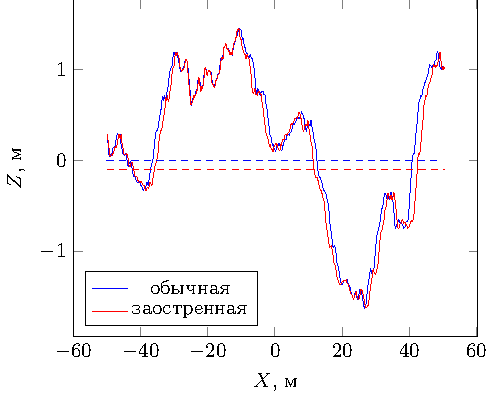
\includegraphics[width=\linewidth]{fig/water/surface_cwm}
        \end{subfigure}
    \end{figure}    
    \begin{minipage}{0.45\linewidth}
        \footnotesize
        \begin{equation}
            \textstyle 
            \begin{gathered} \sigma^2_{\alpha \beta \gamma} =
                \int\limits_{} \frac{\kappa_x^\alpha
                \kappa_y^\beta}{\kappa^{\gamma}} S(\vec \kappa) \dd \vec
                \kappa,\\ \sigma_n^2 = \int\limits_{}^{} \kappa^n S(\vec
                \kappa) \dd \vec \kappa 
            \end{gathered}
        \end{equation}
        \begin{equation}
            \label{eq:char}
            \Theta(\theta) = (1 - i \theta \sigma_1^2 + \theta^2 \Sigma_1)
            \exp(-\frac{1}{2} \theta^2 \sigma_0^2)-
        \end{equation}
        характеристическая функция,
        \end{minipage}
    \hfill
    \begin{minipage}{0.45\linewidth}
        \footnotesize
        \begin{equation}
        \textstyle 
            \tilde P_{\xi_x}(z) = 
            P_{\xi_x}(z)\qty(1 + 
                            \frac{\Sigma_1}{\sigma_0^2} -
                            \frac{\sigma_1^2}{\sigma_0^2} z -
                            \frac{\Sigma_1}{\sigma_0^4}z^2), 
        \end{equation}
        где $P_\xi(z)$ -- гауссовая плотность вероятности наклонов линейной
    поверхности,  $z$ -- высоты морской поверхности.
        \begin{equation}
            \mean{z} = - \sigma_1^2, \quad \mean{z^2} = \sigma_0^2 - 2
            \Sigma_1,
        \end{equation}
        $\Sigma_1 = \sigma^4_{111} - \sigma_{201}^2 \sigma_{021}^2$.
    \end{minipage}
\end{frame}







\begin{frame}[t]
	\frametitle{Форма импульса отраженного от плоской поверхности}
    \begin{figure}[h]
        \centering
        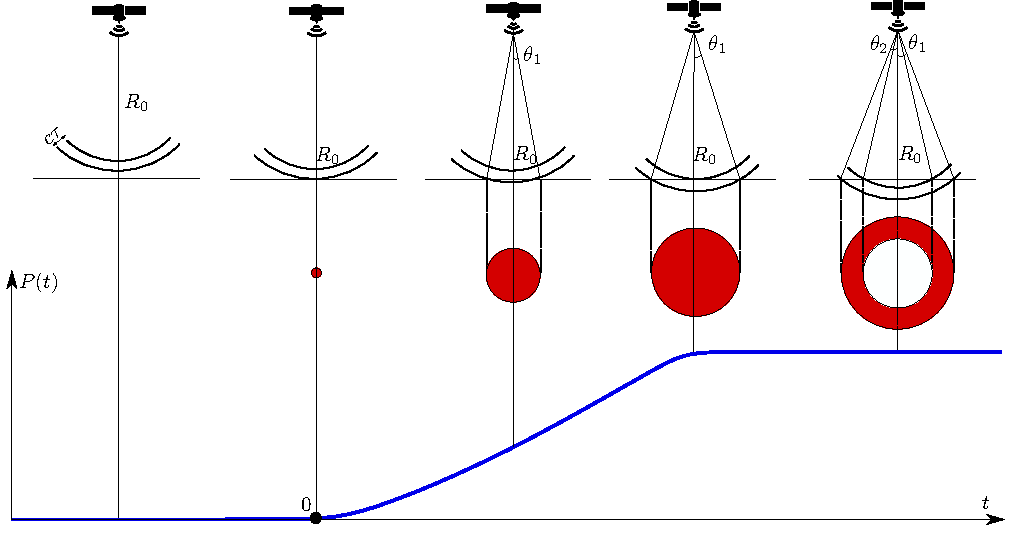
\includegraphics[width=\linewidth]{fig/flat_wave1.pdf}
    \end{figure}
    \footnotesize
    \begin{equation}
        \label{eq:E}
        E = \sum\limits_{i=1}^{M}\frac{E_0}{R_i^2} \exp{-2i\vec k\vec R_i}
        \sigma_i^o 
        G^2(\theta_i)
        , \text{ где}
    \end{equation}
    $R_i$ -- радиус-вектор  от радиовысотомера к рассеивающей площадке,

    $G(\theta)$ -- диаграмма направленности антенны,

    $\sigma^o$ -- сечение обратного рассеяния площадки.
\end{frame}
\begin{frame}[t]
	\frametitle{Геометрия задачи для взволнованной поверхности}
    \begin{minipage}{0.75\linewidth}
    \begin{figure}[h]
        \begin{subfigure}{\linewidth}
            \centering
            \def\svgwidth{\linewidth}
            \includesvg{local_theta}
        \end{subfigure}
    \end{figure}
    \end{minipage}
    \hfill
    \begin{minipage}{0.24\linewidth}
    $(x_0,y_0,z_0)$ -- координаты радиовысотомера

    $(x,y,z)$ -- координата точки на поверхности

    $\zeta_x,\zeta_y$ -- уклоны поверхности по осям $x$ и  $y$

    \end{minipage}

    \begin{equation}
        \cos \theta_0 = \frac{\vec R \vec n}{|\vec R|\abs{\vec n}} - \text{
        локальный угол падения }
    \end{equation}
\end{frame}
\begin{frame}[t]
	\frametitle{Моделирование отраженного импульса}
    \begin{figure}[h]
        \begin{subfigure}{0.60\linewidth}
            \centering
            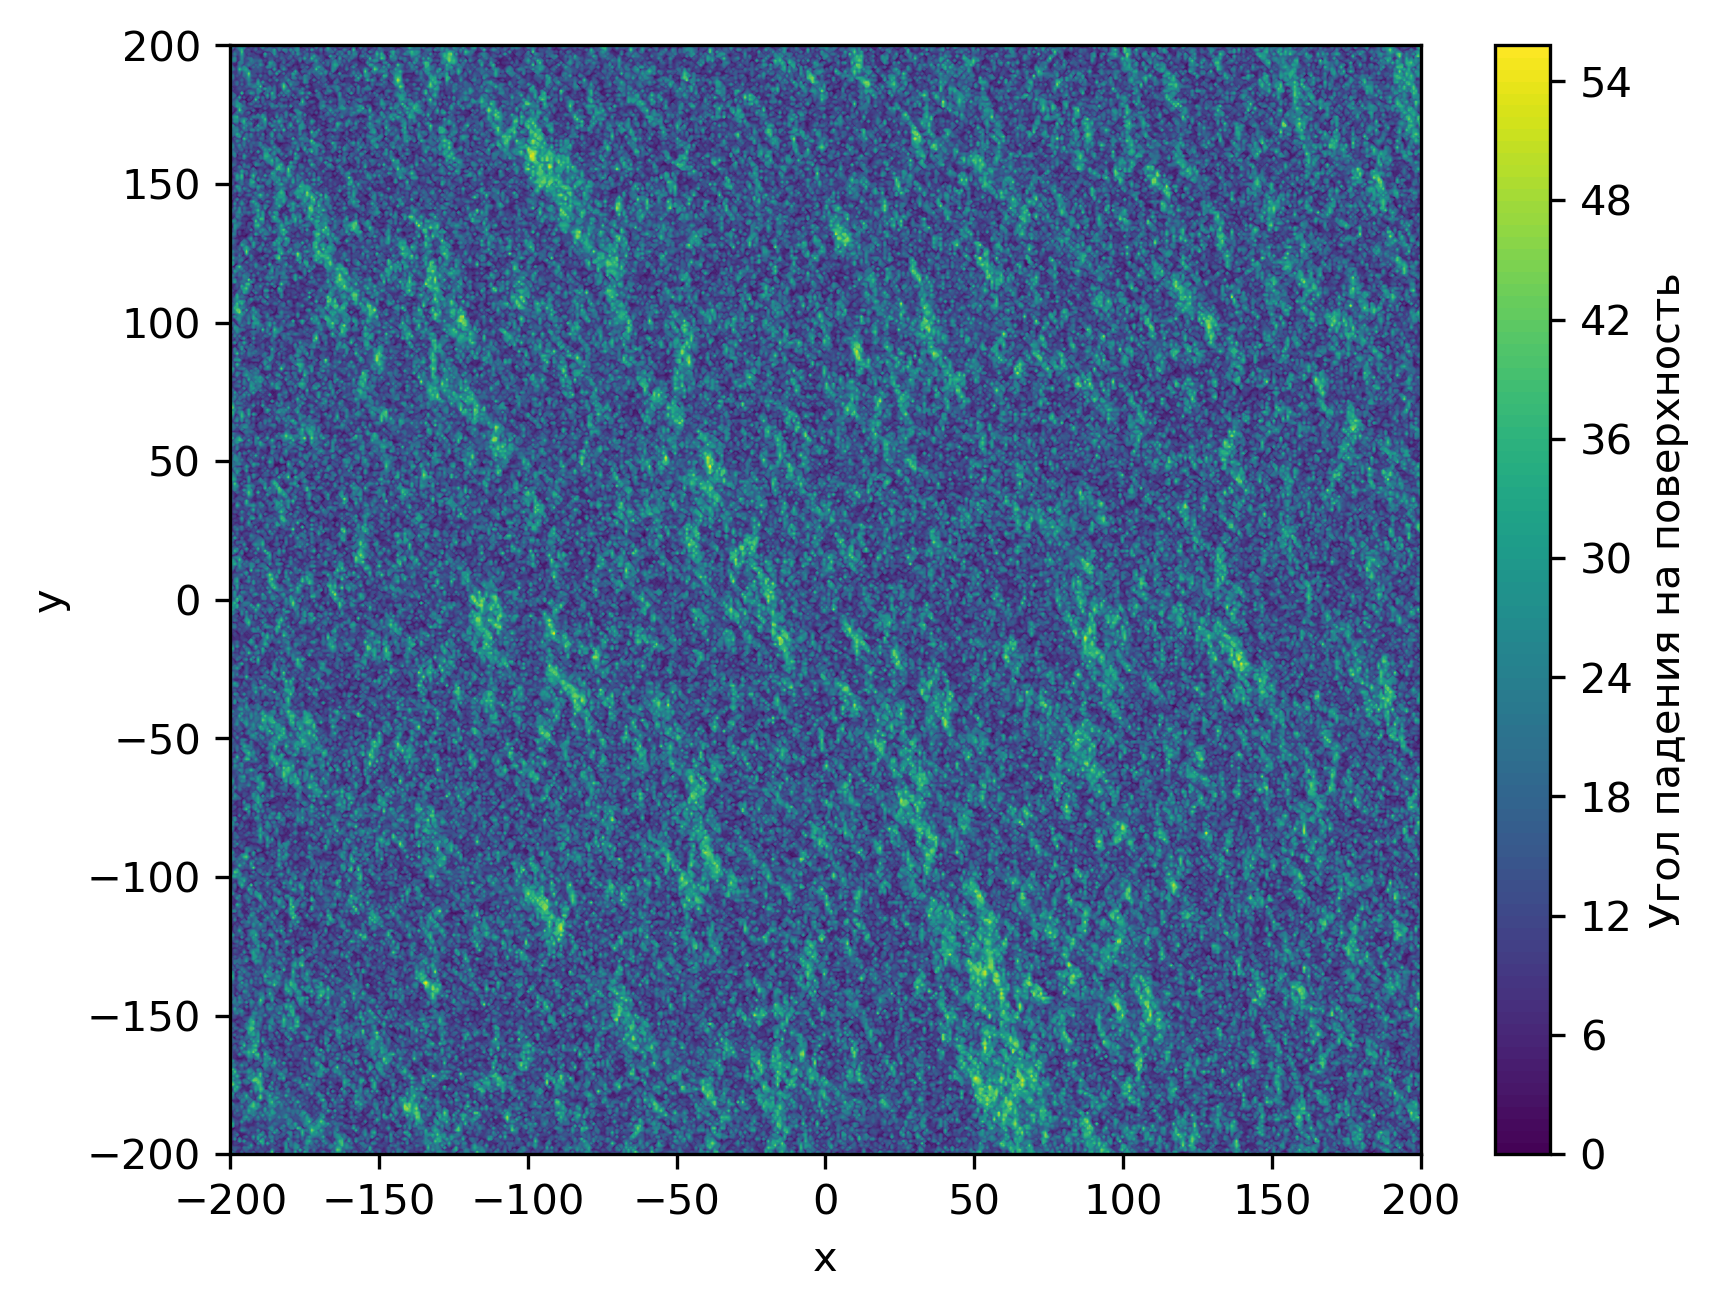
\includegraphics[width=\linewidth]{img/theta0}
        \end{subfigure}
        \begin{subfigure}{0.39\linewidth}
            \centering
            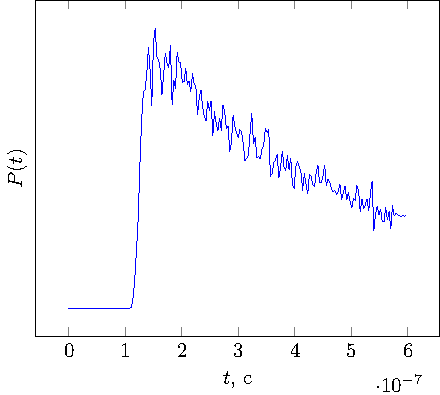
\includegraphics[width=\linewidth]{fig/theta}
        \end{subfigure}
        \caption*{Вычисление локального угла падения
            для радиовысотомера, находящегося в
            точке c координатами $(0,0)$ на высоте 1000 км над уровнем
            моря.  Точки, градусная мера которых меньше $\theta<1^\circ$ в
            дальнейшем будут считаться зеркальными и они будут участвовать в
            формировании отраженного импульса.}
    %\caption*{Форма отраженного импульса в зависимости от времени.}
    \end{figure}
\end{frame}
\begin{frame}[t]
	\frametitle{Моделирование отраженного импульса}
    \begin{equation}
        \label{eq:brown}
        P(t) = A e^{-v} (1 + \erf(u)), \text{ где}
    \end{equation}
    \begin{gather}
        A = A_0 \exp{\frac{- 4}{\gamma} \sin^2 \xi},~
        u = \frac{t - \alpha \sigma_c^2}{\sqrt 2 \sigma_c},~
        v = \alpha\qty(t - \frac{\alpha}{2} \sigma_c^2)~
    \end{gather}
    в которых
    \begin{equation}
        \alpha = \delta - \frac{\beta^2}{4} = \frac{4}{\gamma}\cdot \frac{c}{h} \qty(\cos 2\xi - \frac{\sin^2 2\xi}{\gamma}),
    \end{equation}
    \begin{equation}
        \gamma = \frac{\ln 2}{2} \sin^2 \theta_{-3 dB},
        \sigma_c^2 =  \sigma_p^2 + \frac{\sigma^2}{c^2},
    \end{equation}
    $\xi \ll 1$ -- малое отклонение антенны от надира,  

    $\theta_{-3 dB}$ -- ширина
    диаграммы направленности антенны на уровне $-3dB$, 

    $h$ -- высота радиолокатора над поверхностью земли, 

    $c$ -- скорость света в вакууме, 

    $\sigma^2$ -- дисперсия высот взволнованной морской поверхности.


	%\hfill
	%\begin{minipage}{0.5\linewidth}
        %\begin{equation}
            %P(t) = A \exp{S_T(t - \frac{\tau}{2}) \qty(1 + \erf\frac{t -
        %\tau}{\sigma_L})}
        %\end{equation}
	%\end{minipage}
\end{frame}

\begin{frame}[t]
	\frametitle{Моделирование отраженного импульса}
\begin{equation}
    \label{eq:ice}
    P(t) = A \exp{ S_T (t - \frac{\tau}{2})} \qty(1 + \erf{\frac{t-
    \tau}{\sigma_L}}), \text{ где}
\end{equation}

 $S_T$ -- коэффициент наклона заднего фронта импульса, 

 $\tau$ -- эпоха,

 $\sigma_L$ -- ширина переднего фронта импульса, 

    \begin{figure}[h]
        \centering
        \def\svgwidth{0.8\linewidth}
        \includesvg{example_impulse1}
        %\caption{Качественная форма импульса с обозначением основных параметров.}
        \label{fig:impuls}
    \end{figure}
\end{frame}


% \begin{frame}[t]\frametitle{Модель поверхностного волнения}
    
% \begin{figure}[h!]
% \begin{minipage}[h]{0.45\linewidth}
% 	\centering
% 	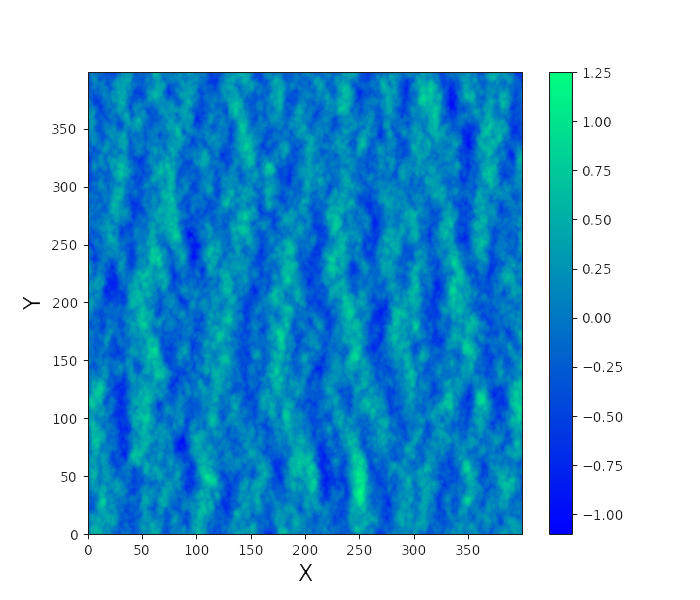
\includegraphics[width=\linewidth]{img/water7.png}
% 	% \caption{Моделирование высот морского волнения. $N=256, ~ U_{10}=7$  }
% 	\label{fig:water7}
% \end{minipage}
% \hfill
% \begin{minipage}[h]{0.45\linewidth}
% 	\centering
% 	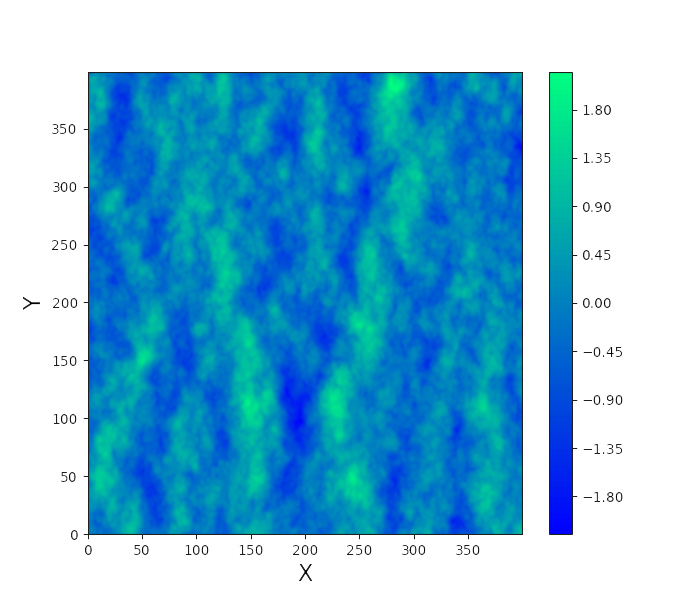
\includegraphics[width=\linewidth]{img/water10.png}
% 	% \caption{Моделирование высот морского волнения. $N=256, ~ U_{10}=10$ }
% 	\label{fig:water10}
% \end{minipage}
% \end{figure}

% \end{frame}
\begin{frame}
\frametitle{Алгоритм ретрекинга}
\vskip -3pt
\def\imp{fig/retracking}
\begin{figure}
    \centering
    \begin{subfigure}{0.49\linewidth}
    При $t > t_{max}$ 
    \begin{equation}
        P(t) = 2A\exp{S_T\qty(t - \frac{\tau}{2})}
    \end{equation}
        \centering
        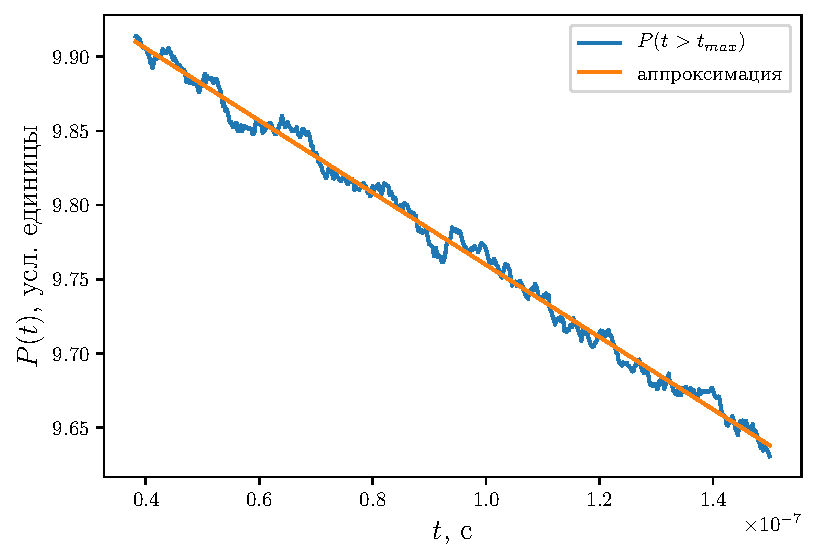
\includegraphics[width=1\linewidth]{\imp/imp_5_1}
        \begin{equation}
            \footnotesize
            \ln P(t) = \ln 2A + S_T(t - \frac{\tau}{2}) = S_T t + const
        \end{equation}
    \end{subfigure}
    \hfill
    \begin{subfigure}{0.49\linewidth}
        При $t < t_{max}$ 
        \begin{equation}
            \dv{\erf\frac{t - \tau}{\sigma_L}}{t} \gg 
            \dv{\exp{S_T(t - \frac{\tau}{2})}}{x}
        \end{equation}

        \centering
        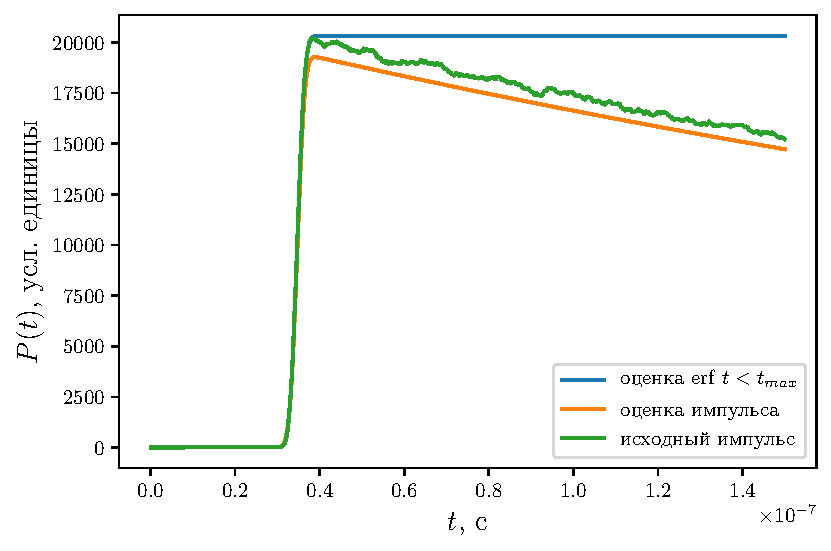
\includegraphics[width=1\linewidth]{\imp/imp_5_2}
        \begin{equation}
            \footnotesize
            P(t) \approx A\qty(1 + \erf\frac{t - \tau}{\sigma_L})
        \end{equation}
    \end{subfigure}

\end{figure}
\end{frame}

\begin{frame}
    %\begin{subfigure}{0.49\linewidth}
        %\centering
        %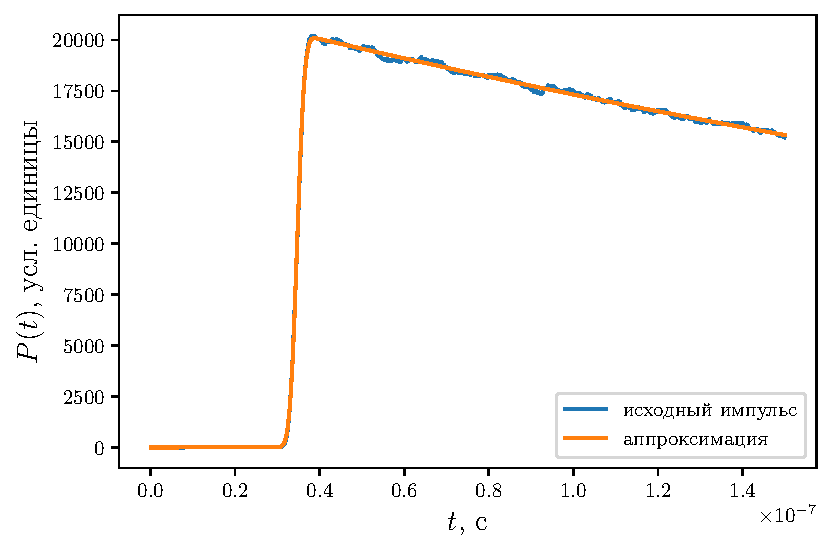
\includegraphics[width=1\linewidth]{\imp/imp_5_3}
    %\end{subfigure}
\frametitle{Ретрекинг модельных импульсов}
\vskip -3pt
\begin{figure}
    \centering
    \begin{subfigure}{0.42\linewidth}
        \centering
        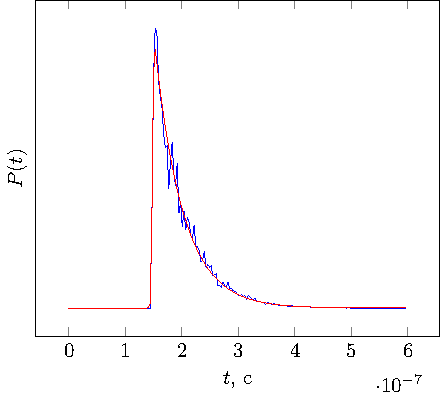
\includegraphics[width=1\linewidth,page=1]{fig/retracking/model}
    \end{subfigure}
    \hfill
    \begin{subfigure}{0.42\linewidth}
        \centering
        \includegraphics[width=1\linewidth,page=2]{fig/retracking/model}
    \end{subfigure}
    \hfill
    \begin{subfigure}{0.42\linewidth}
        \centering
        \includegraphics[width=1\linewidth,page=3]{fig/retracking/model}
    \end{subfigure}
    \hfill
    \begin{subfigure}{0.42\linewidth}
        %\centering
        \begin{tabular}{|c|c|c|c|}
            \hline
            $h$, м      & $0.83$ & $1.36$ & $5.14$\\
            $\tilde h,$ м & $0.65$ & $1.49$ & $4.9$\\
            \hline
        \end{tabular}

        \vspace{\baselineskip}

        $h$ -- высота, заложенная в моделировании

        $\tilde h$ -- высота, полученная нами

        Усредненная по 100 импульсам относительная погрешность измерения
        составляет 10-15\%.
    \end{subfigure}

\end{figure}
\end{frame}

\begin{frame}
\frametitle{Ретрекинг импульсов с Jason-3}
\vskip -3pt
\begin{figure}[ht]
    \centering
    \begin{subfigure}{\linewidth}
        \centering
        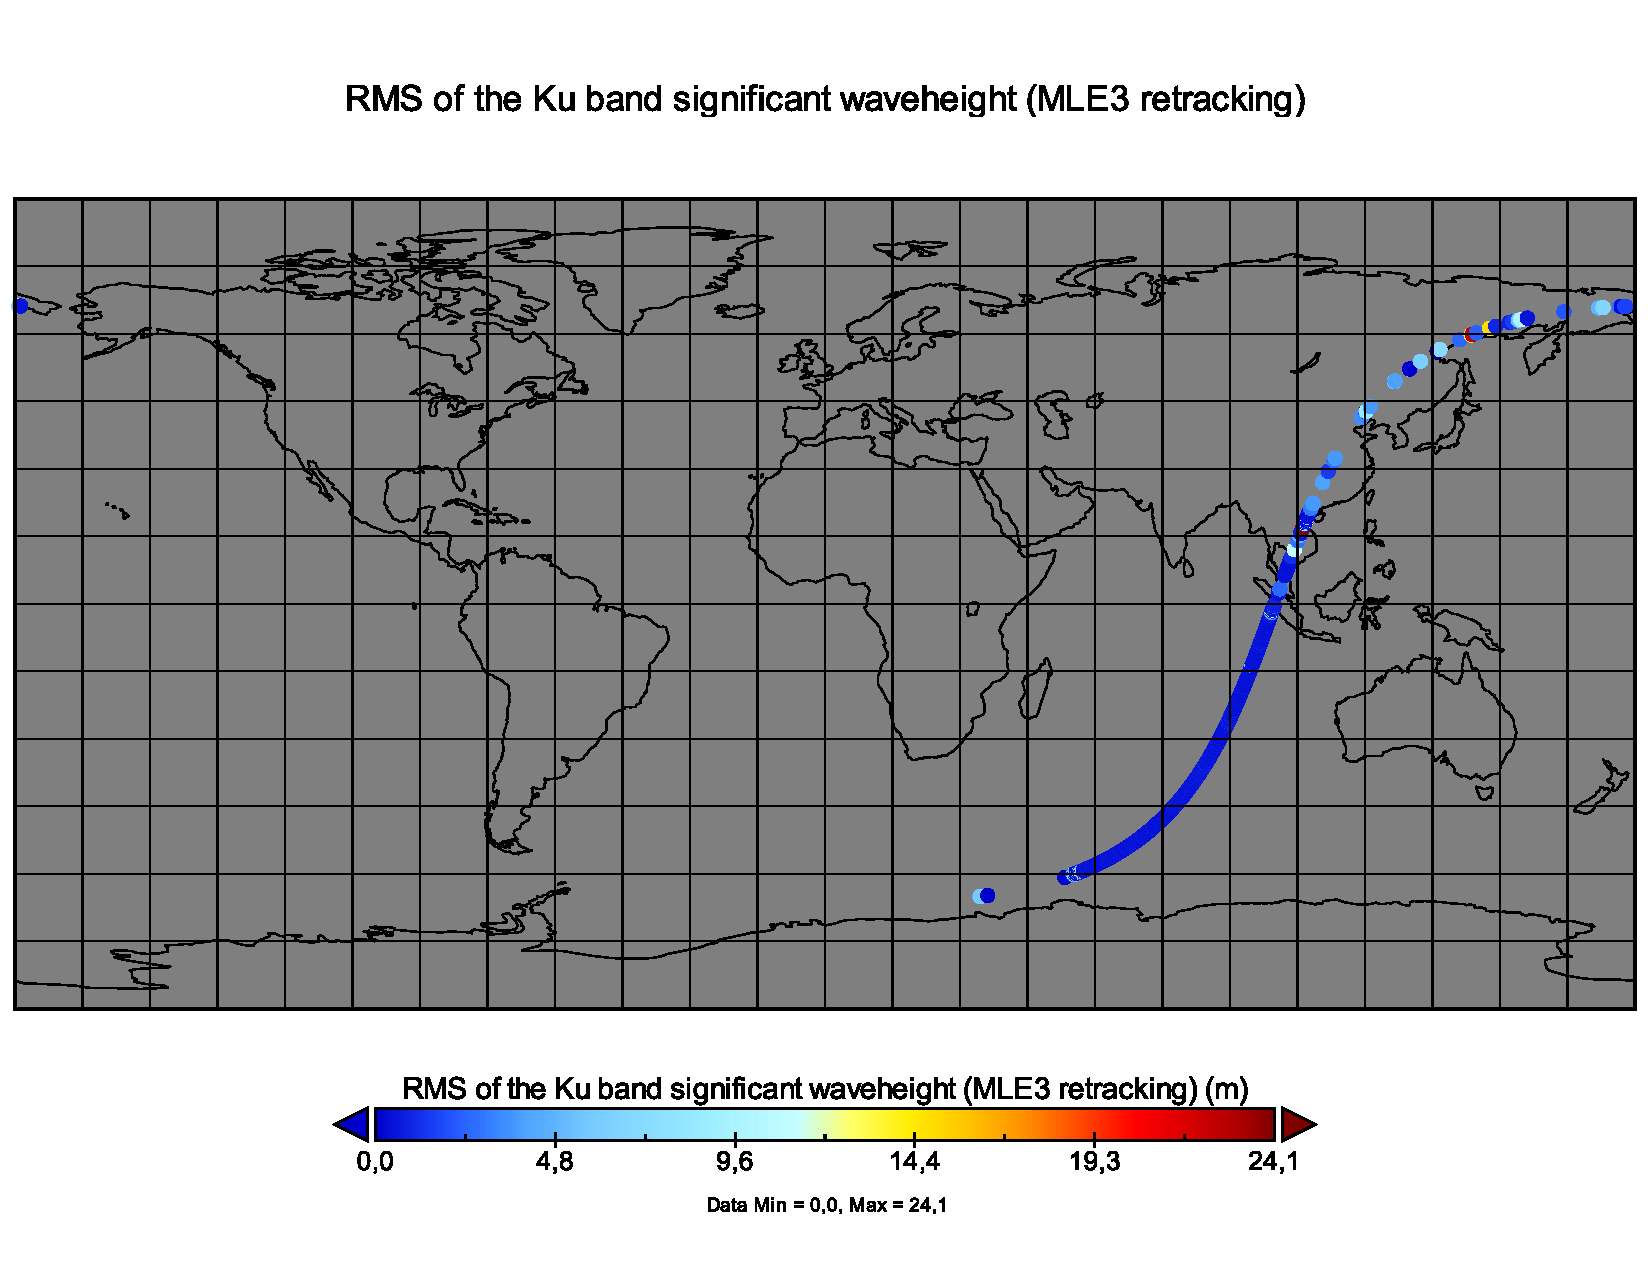
\includegraphics[width=\linewidth]{img/swh_rms_ku_mle3}
    \end{subfigure}
\end{figure}
\end{frame}
\begin{frame}
\frametitle{Ретрекинг импульсов с Jason-3}
\vskip -3pt
\begin{figure}[ht]
    \centering
    \begin{subfigure}{\linewidth}
        \centering
        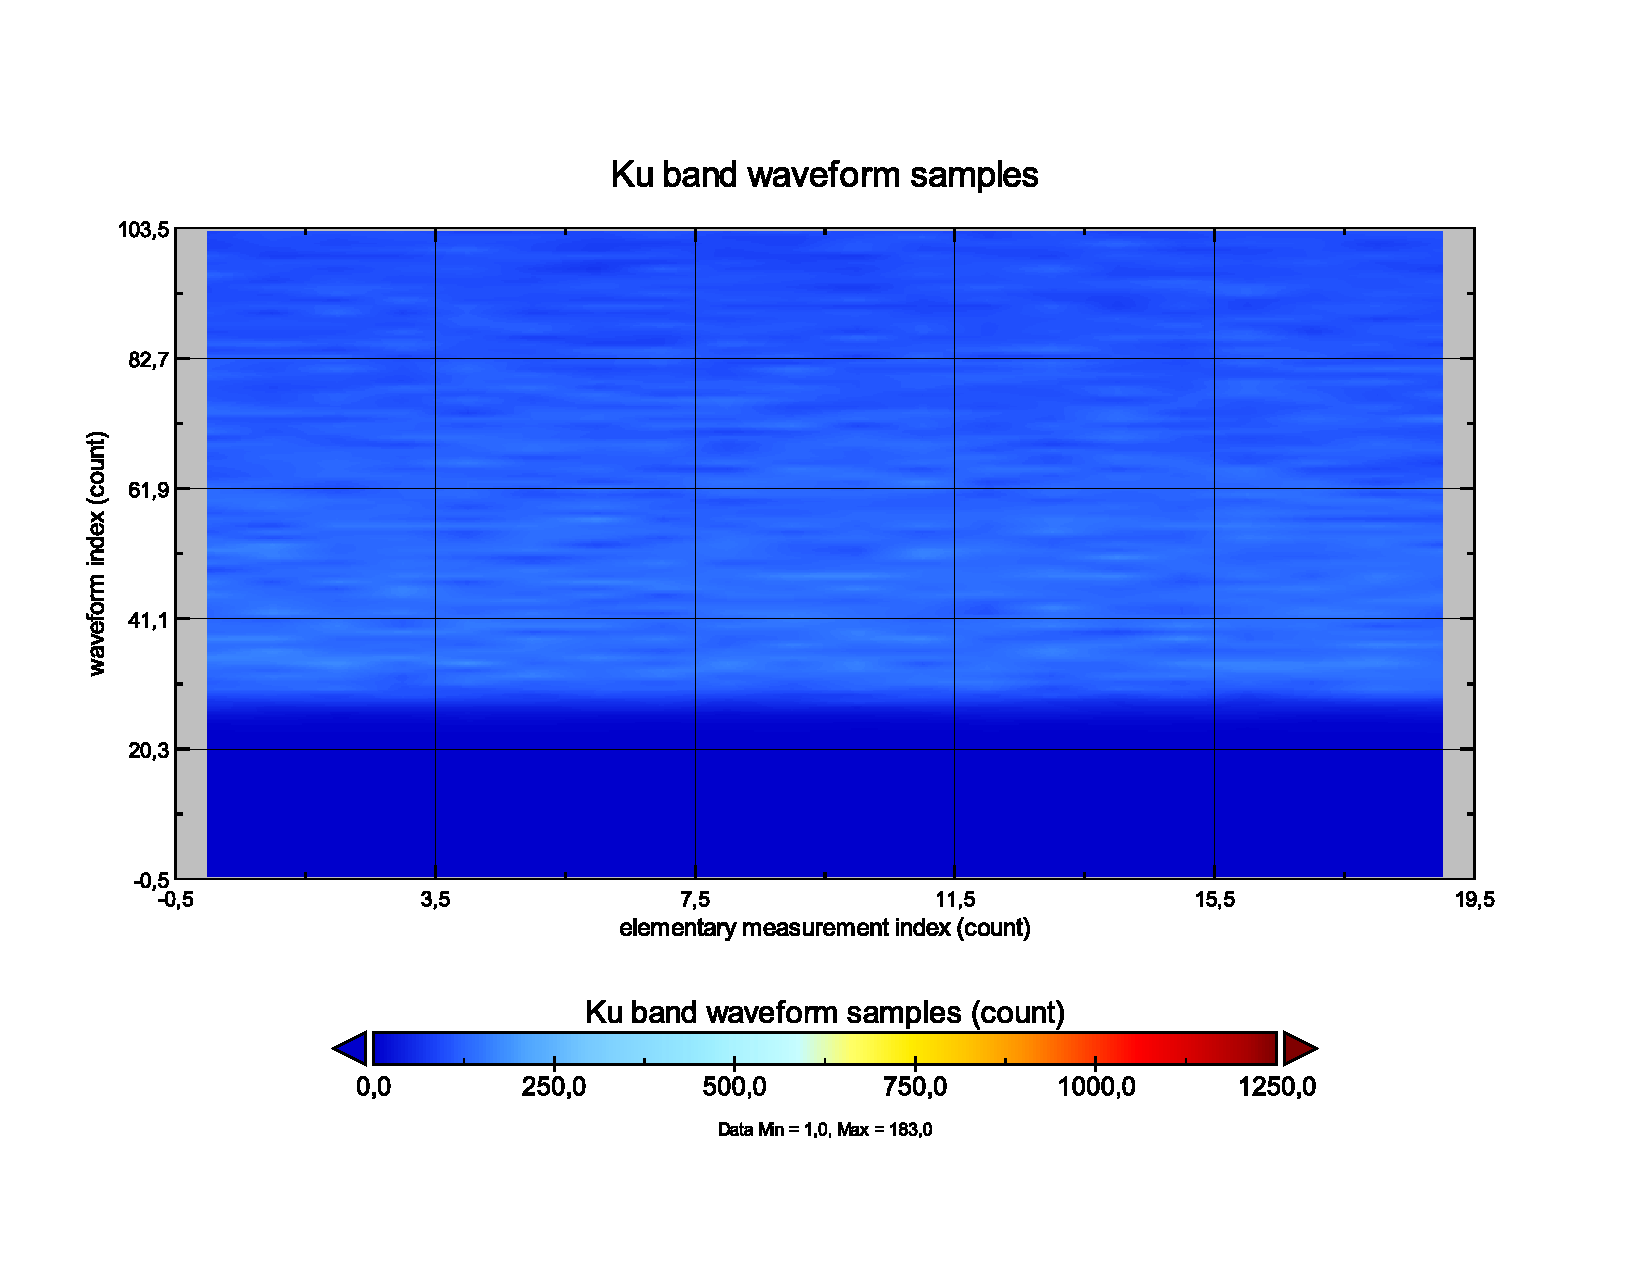
\includegraphics[width=\linewidth]{img/waveforms_20hz_ku.pdf}
    \end{subfigure}
\end{figure}
\end{frame}
\begin{frame}
\frametitle{Ретрекинг импульсов с Jason-3}
\vskip -3pt
\begin{figure}[ht]
    \centering
    \begin{subfigure}{0.42\linewidth}
        \centering
        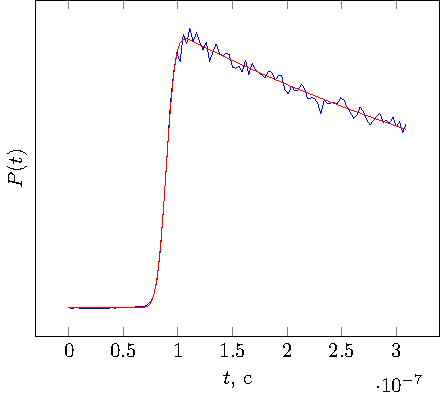
\includegraphics[width=\linewidth, page=1]{fig/retracking/real}
    \end{subfigure}
    \hfill
    \begin{subfigure}{0.42\linewidth}
        \centering
        \includegraphics[width=\linewidth, page=2]{fig/retracking/real}
    \end{subfigure}
    \hfill
    \begin{subfigure}{0.42\linewidth}
        \centering
        \includegraphics[width=\linewidth, page=3]{fig/retracking/real}
    \end{subfigure}
    \hfill
    \begin{subfigure}{0.42\linewidth}
        \centering
        \begin{tabular}{|c|c|c|c|}
            \hline
            $h$, м      & $0.937 $ & $0.699$ & $1.075$ \\
            $\tilde h,$ м & $0.931$ & $0.703$ & $1.081$ \\
            \hline
        \end{tabular}

        \vspace{\baselineskip}

        $h$ -- высота, полученная NASA

        $\tilde h$ -- высота, полученная нами

    Усредненная по 100 импульсам относительная погрешность измерения
    составляет $<2\%$.
    \end{subfigure}
    %\caption{Форма отраженного импульса в зависимости от времени, полученного с
    %радиовысотомера космической миссии Jason-3.}

\end{figure}
\end{frame}

\begin{frame}[t]
	\frametitle{Заключение}
	\vfill
    В настоящей работе были:
		\begin{enumerate}
			\item Изучены принципы моделирования морской поверхности

			\item Предложены способы приближения модельной поверхности к
                реальной

			\item Предложены способы оптимизации времени моделирования
		\end{enumerate}
		\vfill

    Применение модели:

	\begin{enumerate}
		% \item Проведение испытаний оборудования до его изготовления
		\item Тестирование и разработка алгоритмов восстановления океанографической информации
		\item Оценка возможностей новых радиолокаторов
		\item Постановка численных экспериментов
	\end{enumerate}
	\vfill

    Дальнейшие планы: 
	\begin{enumerate}
        %\item \sout{Заварить кофе}
		\item Модификация метода заостренной волны
        \item Учет при моделировании атмосферы и ионосферы
	\end{enumerate}
	\vfill
    
\end{frame}


\end{document}
